\documentclass[11pt]{article}
\RequirePackage{fullpage}
\RequirePackage[font=small,labelfont=bf]{caption}
\RequirePackage{amsmath,amssymb,amsthm}
\RequirePackage{mathtools}
\RequirePackage{tabularx}
\RequirePackage{graphicx}
\RequirePackage[normalem]{ulem}
\RequirePackage[hidelinks]{hyperref}
\RequirePackage{wrapfig}
\RequirePackage{subcaption}
\RequirePackage{authblk}
\RequirePackage{bm}
\RequirePackage{bbm}
\RequirePackage{tikz}
\RequirePackage{wrapfig}


% line numbers:
\RequirePackage{lineno}
% \modulolinenumbers[5]
\linenumbers
\renewcommand\linenumberfont{\normalfont\tiny\sffamily\color{black}}

% spacing
\RequirePackage{setspace}
% \doublespacing
 
% \RequirePackage[osf]{mathpazo}
\RequirePackage[bibstyle=authoryear,citestyle=authoryear-comp,
                date=year,
                maxbibnames=9,maxnames=5,maxcitenames=2,
                backend=biber,uniquelist=false,uniquename=false,
                % style=apa,
                sorting=nyt,
                % sorting=,
                hyperref=true]{biblatex}
\RequirePackage[colorinlistoftodos]{todonotes}  %disable
\RequirePackage{color}
\RequirePackage{nicefrac}

\newcommand{\gc}[1]{{\it \color{red} #1 } }
\newcommand{\vb}[1]{{\it \color{blue} #1}}
\newcommand{\vbout}[1]{{\it \color{blue} \sout{#1}}}

% a /nonumber you can turn on/off
\newcommand{\nnn}{\nonumber}
%\newcommand{\nnn}{}

\newcommand{\beginsupplement}{%
        \setcounter{table}{0}
        \renewcommand{\thetable}{S\arabic{table}}%
        \setcounter{figure}{0}
        \renewcommand{\thefigure}{S\arabic{figure}}%
     }

\newcommand{\Newnameref}[1]{\textit{\nameref{#1}}}

\renewbibmacro{in:}{}
\AtEveryBibitem{\clearlist{language}}

\newcommand{\graham}[1]{\todo[size=\scriptsize, color=red!50]{#1}}
\newcommand{\vince}[1]{\todo[size=\scriptsize, color=blue!50]{#1}}

\renewcommand{\P}{\mathbb{P}}
\newcommand{\E}{\mathbb{E}}
\newcommand{\V}{\text{V}}
\newcommand{\cf}{\emph{cf.} }
\DeclareMathOperator{\var}{Var}
\DeclareMathOperator{\cov}{Cov}
\DeclareMathOperator{\flt}{\mathrm{flat}}
\DeclareMathOperator{\T}{{\mathrm{T}}}
\newcommand{\logt}{\log_{10}}

\newcommand{\chapquote}[2]{\begin{quotation} \textit{#1} \end{quotation} \begin{flushright} - #2\end{flushright} }

\addbibresource{biblio.bib}


\title{Why do species get a thin slice of $\pi$? Revisiting Lewontin's Paradox of Variation}

\author{Vince Buffalo}
\affil[]{\footnotesize University of Oregon, Institute of Ecology and Evolution\\Eugene, Oregon \\ \href{mailto:vsbuffalo@gmail.com}{vsbuffalo@gmail.com}}

\begin{document}
\maketitle


% Neutral theory predicts that genetic diversity increases with population size,
% yet observed levels of diversity across species vary only two orders of
% magnitude while population sizes likely vary over several. The causes of this
% discrepancy, known as Lewontin's Paradox of Variation, remain unknown. Here I
% revisit Lewontin's Paradox by quantifying the relationship between pairwise
% diversity and approximate census size for 172 metazoan species. Using
% phylogenetic comparative methods, I show this relationship is significant
% accounting for phylogeny, but has high phylogenetic signal and some lineages
% experience shifts in diversity deep in the past. I find a negative relationship
% between recombination map length and census size, suggesting abundant species
% have less recombination and could experience greater reductions in diversity
% due to linked selection. However, I show that even using strong selection
% parameter estimates, models of linked selection are unlikely to explain the
% observed relationship between diversity and census sizes across species.

\begin{abstract} 
  Under neutral theory, genetic diversity in an equilibrium population
  is expected to increase with population size. However, observed levels of
  diversity across metazoans vary only two orders of magnitude, while census
  population sizes ($N_c$) are expected to vary over several. This unexpectedly
  narrow range of diversity is a longstanding enigma in evolutionary genetics
  known as Lewontin's Paradox of Variation (1974). Since Lewontin's
  observation, it has been argued that selection constrains diversity across
  species, yet tests of this hypothesis seem to fall short of explaining the
  orders-of-magnitude reduction in diversity observed in nature. In this work,
  I revisit Lewontin's Paradox and assess whether current models of linked
  selection are likely to constrain diversity to this extent.  To quantify the
  discrepancy between pairwise diversity and census population sizes across
  species, I combine genetic data from 172 metazoan taxa with estimates of
  census sizes from geographic occurrence data and population densities
  estimated from body mass.  Next, I fit the relationship between
  previously-published estimates of genomic diversity and these approximate
  census sizes to quantify Lewontin's Paradox. While previous across-taxa
  population genetic studies have avoided accounting for phylogenetic
  non-independence, I use phylogenetic comparative methods to investigate the
  diversity census size relationship, estimate phylogenetic signal, and explore
  how diversity changes along the phylogeny. I consider whether the reduction
  in diversity predicted by models of recurrent hitchhiking and background
  selection could explain the observed pattern of diversity across species.
  Since the impact of linked selection is mediated by recombination map length,
  I also investigate how map lengths vary with census sizes. I find species
  with large census sizes have shorter map lengths, leading these species to
  experience greater reductions in diversity due to linked selection. Even
  after using high estimates of the strength of sweeps and background
  selection, I find linked selection likely cannot explain the shortfall
  between predicted and observed diversity levels across metazoan species.
  Furthermore, the predicted diversity under linked selection does not fit the
  observed diversity--census-size relationship, implying that processes other
  than background selection and recurrent hitchhiking must be limiting
  diversity.  

\end{abstract}

A longstanding mystery in evolutionary genetics is that the observed levels of
genetic variation across sexual species are confined to an unexpectedly narrow
range. Under neutral theory, the average number of nucleotide differences
between lineages (pairwise diversity, $\pi$) is determined by the balance of
new mutations and their loss by genetic drift
\parencite{Kimura1964-ul,Malecot1948-zv,Wright1931-fl}. In particular, the
expected diversity at neutral sites in a panmictic population of $N_c$ diploids
is expected to be $\pi \approx 4N_c \mu$, where $\mu$ is per generation
mutation rate. Given that metazoan germline mutation rates only differ 10-fold
($10^{-8}$--$10^{-9}$, \cite{Kondrashov2010-fi,Lynch2010-ki}), and census sizes
vary over several orders of magnitude, one would expected under neutral theory
that heterozygosity should also vary over several orders of magnitude. However,
early allozyme surveys revealed that heterozygosity levels across a wide range
of species varied just an order of magnitude \parencite[][p.
208]{Lewontin1974-jb}; this anomaly is known as Lewontin's ``Paradox of
Variation". With modern sequencing-based estimates of $\pi$ across taxa ranging
over only three orders of magnitude ($0.01$--$10\%$, \cite{Leffler2012-zj}),
Lewontin's paradox has persisted unresolved through the genomics era.

From the beginning, explanations for Lewontin's Paradox have been framed in
terms of the neutralist--selectionist controversy
\parencite{Lewontin1974-jb,Kimura1984-ia,Gillespie1991-qa,Gillespie2001-mv}.
The neutralist view is that beneficial alleles are sufficiently rare and
deleterious alleles removed sufficiently quickly, that levels of genetic
diversity are shaped predominantly by genetic drift and mutation
\parencite{Kimura1984-ia}. Specifically, \emph{non-selective} processes
decouple the effective population size implied by observed levels of diversity
$\widehat{\pi}$, $\widetilde{N}_e = \nicefrac{\widehat{\pi}}{4\mu}$, from the
census size, $N_c$. By contrast, the selectionist view is that the direct and
indirect effects of linked selection suppress diversity levels across taxa,
specifically because the impact of linked selection is greater in large
populations. Undoubtedly, these opposing views represent a false dichotomy, as
population genomic studies have uncovered complex demographic histories that
impact diversity within a species (e.g. \cite{Zhao2013-vd,Palkopoulou2015-bg}),
as well as evidence that selection depresses genome-wide diversity (e.g.
\cite{Elyashiv2016-vt,Begun1992-ey,Aguade1989-jx,McVicker2009-ax}). 

\subsection*{Possible Explanations of Lewontin's Paradox}

A resolution of Lewontin's Paradox would involve a mechanistic description and
quantification of the evolutionary processes that prevent diversity from
scaling with census sizes across species. This would necessarily connect to the
broader literature on the empirical relationship between diversity and
population size
\parencite{Frankham1996-yb,Nei1984-zi,Soule1976-he,Leroy2021-gy}, and the
ecological and life history correlates of genetic diversity
\parencite{Nevo1978-wh,Powell1975-lg,Nevo1984-hp}. Three categories of
processes stand out as potentially capable of decoupling census sizes from
diversity: non-equilibrium demography, variance and skew in reproductive
success, and selective processes.

It has long been appreciated that effective population sizes are typically less
than census population sizes, tracing back to early debates between R.A. Fisher
and Sewall Wright \parencite{Fisher1947-tf,Wright1948-fj}. Possible causes of
this divergence between effective and census population sizes include
demographic history (e.g. population bottlenecks), extinction and
recolonization dynamics, or the breeding structure of populations (e.g. the
variance in reproductive success and population substructure). Early
explanations for Lewontin's Paradox suggested bottlenecks during the last
glacial maximum severely reduced population sizes
\parencite{Kimura1984-ia,Ohta1973-pk,Nei1984-zi}, and emphasized that large
populations recover to equilibrium diversity levels more slowly
(\cite{Nei1984-zi}, \cite{Kimura1984-ia} p. 203-204). Another explanation is
that cosmopolitan species repeatedly endure extinction and recolonization
events, which reduces effective population size
\parencite{Maruyama1980-xz,Slatkin1977-kd}. 

While chance demographic events like bottlenecks and recent expansions have
long-term impacts on diversity (equilibrium is reached on the order of size of
the population), characteristics of the breeding structure such as high
variance ($V_w$) or skew in reproductive success  also suppress diversity below
the levels predicted by the census size \parencite{Wright1938-tv}. In species
like marine animals, females are highly fecund, and dispersing larvae face
extremely low survivorship, leading to high variance in reproductive success
\parencite{Waples2018-kb,Waples2013-wi,Hedgecock2011-ku,Hauser2008-fd}. Such
``sweepstakes" reproductive systems can lead to remarkably small ratios of
effective population size to census population size (e.g. $\nicefrac{N_e}{N_c}$
can range from $10^{-6}$--$10^{-2}$), since $\nicefrac{N_e}{N} \approx
\nicefrac{1}{V_w}$
\parencite{Hedgecock1994-gs,Wright1938-tv,Nunney1993-ef,Nunney1996-wy}, and
require multiple-merger coalescent processes  to describe their genealogies
\parencite{Eldon2006-ui}. Overall, these reproductive systems diminish the
diversity in many species, but seem unlikely to explain Lewontin's Paradox
broadly across metazoans.

Alternatively, selective processes, and in particular the indirect effects of
selection on linked neutral variation, could explain the observed narrow range
of diversity. The earliest mathematical model of hitchhiking was proffered as a
solution to Lewontin's Paradox \parencite{Maynard_Smith1974-zr}.  Since,
empirical observations have demonstrated that linked selection shapes patterns
of genome-wide diversity, as evidenced by the correlation between recombination
and diversity in a variety of species
\parencite{Aguade1989-jx,Begun1992-ey,Cutter2003-tl,Stephan1998-hh,Cai2009-by}.
Theoretic work to explain this pattern has considered diversity under a steady
influx of new beneficial mutations (recurrent hitchhiking;
\cite{Stephan1992-jc,Stephan1995-ry}), and purifying selection against new
deleterious mutations (background selection, BGS;
\cite{Charlesworth1993-gb,Nordborg1996-nq,Hudson1994-oh,Hudson1995-xc}).
Indeed, empirical work indicates background selection diminishes diversity
around genic regions in a variety of species
\parencite{McVicker2009-ax,Hernandez2011-gs,Charlesworth1996-px}, and now
efforts have shifted towards teasing apart the effects of positive and negative
selection on genomic diversity \parencite{Elyashiv2016-vt}.

An important class of theoretic selection models pertaining to Lewontin's
Paradox are recurrent hitchhiking models that decouple diversity from the
census population size. These models predict diversity when strongly selected
beneficial mutations regularly enter and sweep through the population, trapping
lineages and forcing them to coalesce
\parencite{Kaplan1989-sc,Gillespie2000-mh}. In general, decoupling occurs under
these hitchhiking models when the rate of coalescence due to selection is much
greater than the rate of neutral coalescence \parencite[equation
22]{Coop2012-cd}. Other selection models cannot alone decouple diversity from
population size, \emph{ceteris paribus}. For example, the reduction in
diversity predicted under background selection and polygenic fitness variation
is a proportion reduction in population size, mediated by the total
recombination map length
\parencite{Charlesworth1993-gb,Nicolaisen2012-vs,Nordborg1996-nq,Robertson1961-ho,Santiago1995-hx,Santiago1998-bs}.

\subsection*{Recent Approaches Towards Solving Lewontin's Paradox}

Recently, \textcite{Corbett-Detig2015-gt} used population genomic data to
estimate the reduction in diversity due to background selection and hitchhiking
across 40 species, and showed the impact of selection increases with two
proxies of census population size, species range and with body size. These
authors argued this is evidence that selection could explain Lewontin's
Paradox; however, in a re-analysis, \textcite{Coop2016-gx} demonstrated that
the observed scale of these reductions is insufficient to explain the
orders-of-magnitude shortfall between observed and expected levels of diversity
across species. Other recent work has found that certain life history
characteristics related to parental investment, such as propagule size, are
good predictors diversity in animals \parencite{Romiguier2014-bp,Chen2017-nf}.
Nevertheless, while these diversity correlates are important clues, they do not
propose a mechanism by which these traits act to constrain diversity within a
few orders of magnitude. 

Here, I revisit Lewontin's Paradox by integrating a variety of data sets and
assessing the predicted reductions in diversity under different selection
models. Prior surveys of genetic diversity either lacked census population size
estimates, used allozyme-based measures of heterozygosity, or included fewer
species. To address these shortcomings, I first estimate census sizes by
combining predictions of population density based on body size with ranges
estimated from geographic occurrence data. Using these estimates, I quantify
the relationship between census size and previously-published genomic diversity
estimates across 172 metazoan taxa within nine phyla, which provides a sense of
the scale of the divergence between $\pi$ and $N_c$ that leads to Lewontin's
Paradox. 

Past work looking at the relationship between $\pi$ and $N_c$ has largely
ignored phylogenetic non-independence across taxa
\parencite{Felsenstein1985-an}. To address this shortcoming, I account for
phylogenetic non-independence across taxa using a synthetic time-calibrated
phylogeny and phylogenetic comparative methods (PCMs). Moreover,
\textcite{Lynch2011-qv} has argued that since coalescent times are much less
than divergence times, considering phylogenetic non-independence is unnecessary
for traits like effective population size. Using PCMs, I test this conjecture
by estimating phylogenetic signal in the diversity census size relationship,
and investigating how these traits evolve along the phylogeny.

Finally, I explore whether the predicted reductions of diversity under
background selection and recurrent hitchhiking are sufficiently strong 
to resolve Lewontin's Paradox. These predicted reductions in diversity across
species are generously estimated using selection strength parameters from
\emph{Drosophila melanogaster}, a species known to be strongly affected by
linked selection. Given the effects of linked selection are mediated by
recombination map length, I investigate how recombination map lengths vary with
census population size using data from a previously-published survey
\parencite{Stapley2017-fs}. I find map lengths are typically shorter in
large--census-size species, increasing the effects of linked selection in these
species, which might further decouple diversity from census size. Still, I find
the combined impact of these selection models with available parameter
estimates falls short in explaining Lewontin's Paradox, and discuss future
avenues through which the Paradox of Variation could be fully resolved.

\section*{Results}

\subsection*{Estimates of Census Population Size}

\begin{figure}[t!]
  \centering
  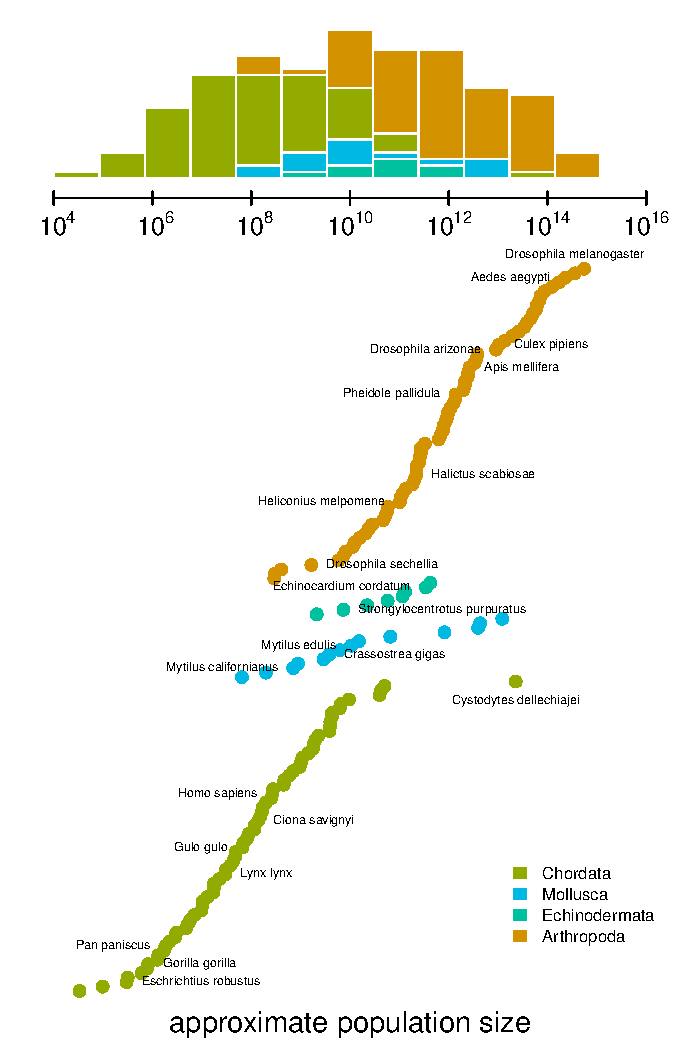
\includegraphics[width=0.6\textwidth]{figures/Nc_figure.pdf}
  \caption{
     The distribution of approximate census population sizes estimated by this
     study. Some phyla containing few species were excluded for clarity.}
\label{fig:figure-nc}
\end{figure}


A major impediment in quantifying Lewontin's Paradox has been estimating census
population sizes across many taxa, especially for extremely abundant,
cosmopolitan species that define the upper limit of ranges. Previous work has
surveyed the literature for census size estimates
\parencite{Nei1984-zi,Soule1976-he,Frankham1996-yb}, or used range and body
size or qualitative categories as proxies for census size
\parencite{Corbett-Detig2015-gt,Leffler2012-zj}. To quantify the relationship
between genomic estimates of diversity and census population sizes, I first
approximate census population sizes for 172 metazoan taxa (Figure
\ref{fig:figure-nc}). My approach predicts population densities from body sizes
using a previously-observed linear relationship that holds across metazoans
(Supplementary Figure \ref{suppfig:damuth};
\cite{Damuth1981-st,Damuth1987-sg}). Then, from geographic occurrence data, I
estimate range sizes. Finally, I estimate population size as the product of
these predicted densities and range estimates (see Methods:
\Newnameref{sec:methods-popsize}). Note that the relationship between
population density and body size is driven by energy budgets, and thus reflects
macroecological equilibria \parencite{Damuth1987-sg}; consequently, population
sizes for taxa like humans and their domesticated species are underestimated.
While these methods to estimate census size are crude and approximate, they can
be efficiently calculated for numerous taxa and are sufficient to estimate the
scale of Lewontin's Paradox.

\subsection*{Quantifying Lewontin's Paradox}

\begin{figure}[t!]
  \centering
  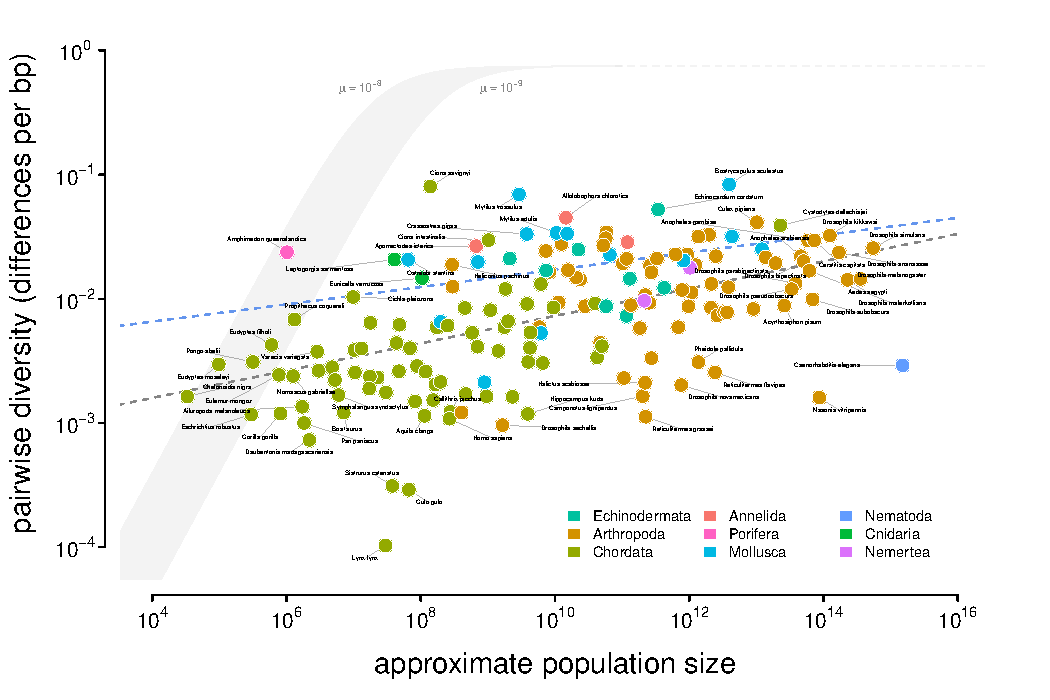
\includegraphics[width=\textwidth]{figures/diversity_popsize_full.pdf}

  \caption{An illustration of Lewontin's Paradox of Variation. Pairwise
    diversity (data from \cite{Leffler2012-zj}, \cite{Corbett-Detig2015-gt},
    and \cite{Romiguier2014-bp}), which varies around three orders of
    magnitude, shows a weak relationship with approximate population size,
    which varies over 12 orders of magnitude.  The shaded curve shows the range
    of expected neutral diversity if $N_e$ were to equal $N_c$ under the
    four-alleles model, $\log_{10}(\pi) = \logt(\theta) - \logt{(1 +
    \nicefrac{4\theta}{3})}$ where $\theta = 4N_c \mu$, for two mutation rates,
    $\mu = 10^{-8}$ and $\mu = 10^{-9}$, and the light gray dashed line
    represents the maximum pairwise diversity under the four alleles model. The
    dark gray dashed line is the OLS regression fit, and the blue
    dashed line is the regression fit using a phylogenetic mixed-effects model.
    Points are colored by phylum.}

  \label{fig:figure-1}
\end{figure}

To determine which ecological or evolutionary processes could decouple
diversity from census population size, we first need to quantify this
relationship across a wide variety of taxa. Previous work has found there is a
significant relationship between heterozygosity and the logarithm of population
size, but these studies relied on heterozygosity measured from allozyme data
\parencite{Soule1976-he,Frankham1996-yb,Nei1984-zi}. Here, I confirm these
findings using pairwise diversity estimates from genomic sequence data and the
estimated census sizes (Figure \ref{fig:figure-1}). The pairwise diversity
estimates are from three sources: \textcite{Leffler2012-zj},
\textcite{Corbett-Detig2015-gt}, and \textcite{Romiguier2014-bp}, and are
predominantly from either synonymous or non-coding DNA (see Methods:
\Newnameref{sec:methods-diversity}). Overall, an ordinary least squares (OLS)
relationship on a log-log scale fits the data well (Figure \ref{fig:figure-1}).
The OLS slope estimate is significant and implies a 0.09 percent increase in
differences per basepair for every order of magnitude census size grows (95\%
confidence interval $[0.08, 0.12]$; see also the OLS fit per-phyla,
Supplementary Figure \ref{suppfig:figure-1-ave}). 

Notably, this relationship has few outliers and is relatively homoscedastic.
This is in part because of the log-log scale, in contrast to previous work
\parencite{Nei1984-zi,Soule1976-he}; see Supplementary Figure
\ref{suppfig:figure-1-linear} for a version on a log-linear scale. However, it
is noteworthy that few taxa have diversity estimates below $10^{-3.5}$
differences per basepair. Those that do, lynx (\emph{Lynx Lynx}), wolverine
(\emph{Gulo gulo}), and Massasauga rattlesnake (\emph{Sistrurus catenatus})
face habitat fragmentation and declining population sizes. These three species
are all in the IUCN Red List, but are listed as least concern (though their
presence in the Red List indicates they are of conservation interest). In
Supplementary Material Section \namref{supinfo:div-iucn}, I explore more about
the relationships between IUCN Red List status, diversity, and population size.

\subsection*{Phylogenetic Non-Independence and the Population Size Diversity Relationship}

In quantifying Lewontin's Paradox, I have additionally fit some simple trait
evolution models that account for phylogenetic non-independence, investigated
whether there is a signal of phylogenetic non-independence, estimated the
continuous trait values on the phylogeny, and assessed how diversity and
population size evolve. Prior population genetic comparative studies have
lacked time-calibrated phylogenies and assumed unit branch lengths
\parencite{Whitney2010-ud}, a shortcoming that has drawn criticism
\parencite{Lynch2011-qv}. Here, I use a synthetic time-calibrated phylogeny
created from the DateLife project \parencite{OMeara2020-ds} to account for
shared phylogenetic history (see Methods: \Newnameref{sec:methods-pcm}).

\begin{figure}[t!]
  \centering
  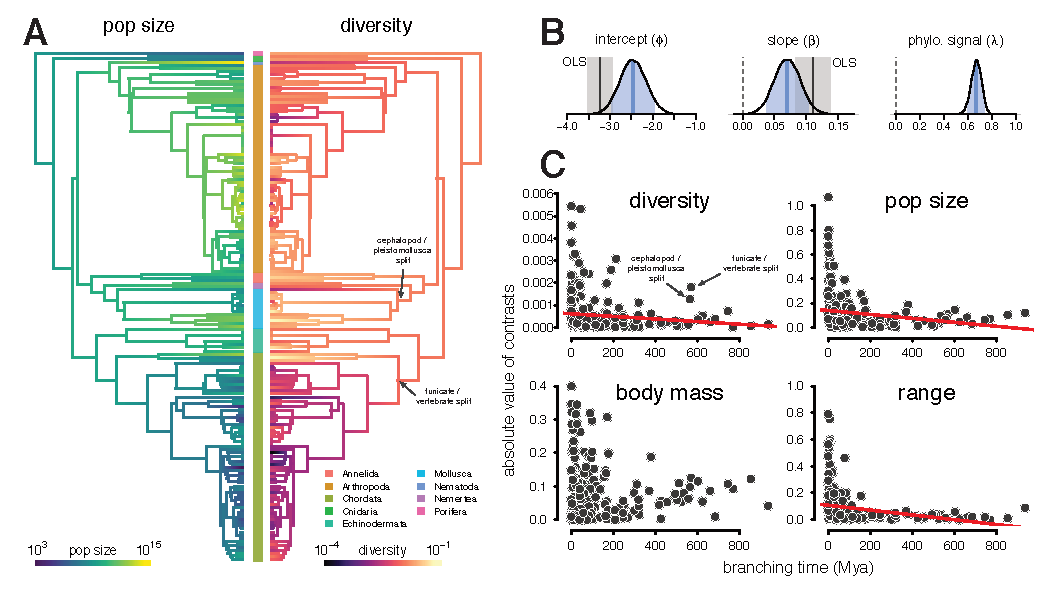
\includegraphics[width=\textwidth]{figures/diversity_pcm.pdf}

  \caption{(A) The ancestral continuous trait estimates for the population size
    and diversity (differences per bp, log scaled) across the phylogeny of 166
    taxa. The phyla of the tips are indicated by the color bar in the center.
    (B) The posterior distributions of the intercept, slope, and phylogenetic
    signal ($\lambda$, \cite{De_Villemereuil2014-kt}) of the phylogenetic
    mixed-effects model of diversity and population size (log scaled). Also
    shown are the 90\% credible interval (light blue shading), posterior mean
    (blue line), OLS estimate (gray solid line), and bootstrap OLS confidence
    intervals (light gray shading).  (C) The node-height tests of diversity,
    population size, and the two components of the population size estimates,
    body mass, and range (all traits on log scale before contrast was
    calculated). Each point shows the standardized phylogenetic independent
    contrast and branching time for a pair of lineages. Red lines are robust
    regression estimates (and are only shown for statistically significant
    relationships at the $\alpha = 0.05$ level). Note that some outlier pairs
    with very high phylogenetic independent contrasts were excluded (in all
    cases, these outliers were in the genus \emph{Drosophila}).}

  \label{fig:figure-2}
\end{figure}


Using a phylogenetic mixed-effects model
\parencite{Lynch1991-tp,Hadfield2010-ql,De_Villemereuil2014-kt} implemented in
Stan \parencite{Carpenter2017-xi,Stan_Development_Team2020-ea}, I estimated the
linear relationship between diversity and population size (on a log-log scale)
accounting for phylogeny, for the 166 taxa with non-missing data and present in
the synthetic chronogram. As with the non-phylogenetic regression, this
relationship was positive and significant (95\% credible interval $0.04,
0.11$), though somewhat attenuated compared to the OLS estimates (Figure
\ref{fig:figure-2}B). Since the population size estimates are based on range
and body mass, they are essentially a composite trait; fitting phylogenetic
mixed-effects models separately on body mass and range indicates these have
significant negative and positive effects, respectively (Supplementary Figure
\ref{suppfig:figure-div-range-bodymass}).

With the phylogenetic mixed-effects model, I also estimated the variance of the
phylogenetic effect ($\sigma_p^2$) and the residual variance ($\sigma_r^2$),
which can be used to estimate a measure of the phylogenetic signal, $\lambda =
\nicefrac{\sigma_p^2}{(\sigma_p^2 + \sigma_r^2)}$
(\cite{Lynch1991-tp,De_Villemereuil2014-kt}; see \cite{Freckleton2002-ly} for a
comparison to Pagel's $\lambda$).  If the relationship between diversity and
population size was free of shared phylogenetic history, $\lambda = 0$ and all
the variance could be explained by evolution on the tips; this is analogous to
Lynch's conjecture that coalescent times should be free of phylogenetic signal
(\citeyear{Lynch2011-qv}). In the relationship between population size and
diversity, the posterior mean of $\lambda = 0.67$ (90\% credible interval
$[0.59, 0.75]$) indicates that the majority of the variance perhaps might be
due to shared phylogenetic history (Figure \ref{fig:figure-2}B).

A closer visual inspection of the estimated ancestral continuous values for
diversity and population size on the phylogeny indicates the high phylogenetic
signal seems to be driven in part by chordates having low diversity and small
population sizes compared to non-chordates (Figure \ref{fig:figure-2}A). This
suggests \citeauthor{Gillespie1991-qa}'s (1991) earlier critique that the
$\pi$--$N_c$ relationship was driven by chordate-arthropod differences may be
valid. This problem resembles Felsenstein's worst-case scenario
\parencite{Felsenstein1985-an,Uyeda2018-wf}, where a singular event on a
lineage separating two clades generates a spurious association between two
traits. To further investigate whether clade-level differences dominated the
relationship between diversity and population size, I fit phylogenetic
mixed-effects models to phyla-level subsets of the data for clades with
sufficient sample sizes (see Methods: \Newnameref{sec:methods-pcm}). This
analysis shows a significant positive relationship between diversity and
population size in arthropods, and positive weak relationships in molluscs and
chordates (Supplementary Figure \ref{suppfig:div_popsize_post_phyla}). Each of
the 90\% credible intervals for slope overlap, indicating the relationship
between $\pi$ and $N_c$ is similar across these clades.

One limitation of the phylogenetic mixed-effects models employed here is that
they assume traits evolve under constant-rate Brownian motion. To test this
assumption, I performed node-height tests \parencite{Freckleton2006-ww}.
Node-height tests regress the absolute values of the standardized contrasts
between lineages against the branching time (since present) of these lineages.
Under Brownian Motion (BM), standardized contrasts are estimates of the rate of
character evolution \parencite{Felsenstein1985-an}; if a trait evolves under
constant rate BM, this relationship should be flat. For both diversity and
population size, node-height tests indicate a significant increase in the rate
of evolution towards the present (robust regression p-values 0.028 and 0.00070
respectively; Figure \ref{fig:figure-2}C).  Considering the constituents of the
population size estimate, range and body mass, separately, the rate of
evolution of range but not body mass shows a significant increase (p-value $1.9
\times 10^{-7}$) towards the present. 

Interestingly, the diversity node-height test reveals two rate shifts at deeper
splits (Figure \ref{fig:figure-2}C, top left) around 570 Mya. These nodes
represent the branches between tunicates and vertebrates in chordates, and
cephalopods and pleistomollusca (bivalves and gastropods) in molluscs.  While
the cephalopod-pleistomollusca split outlier may be an artifact of having a
single cephalopod (\emph{Sepia officinalis}) in the phylogeny, the
tunicate-vertebrate split outlier is driven by the low diversity of vertebrates
and the previously-documented exceptionally high diversity of tunicates (sea
squirts; \cite{Nydam2010-kg,Small2007-mt}). This deep node representing a rate
shift in diversity could reflect a change in either effective population size
or mutation rate, and there is some evidence of both in this genus \emph{Ciona}
\parencite{Small2007-mt,Tsagkogeorga2012-lv}. Neither of these deep rate shifts
in diversity is mirrored in the population size node-height test (Figure
\ref{fig:figure-2}C, top right). Rather, it appears a trait impacting diversity
but not census size (e.g. mutation rate or offspring distributions) has
experienced a shift on the lineage separating tunicates and vertebrates. At
nearly 600 Mya, these deep nodes illustrate a counterexample to Lynch's claim
that expected coalescent times do not share phylogenetic history because they
are less than divergence times. 

Finally, an important caveat is the increase in rate towards the tips could be
caused by measurement noise. Inspecting the lineage pairs that lead to this
increase in rate towards the tips indicates these represent plausible rate
shifts, e.g. between cosmopolitan and endemic sister species like
\emph{Drosophila simulans} and \emph{Drosophila sechellia}; however, ruling out
measurement noise entirely as an explanation would involve considering the
uncertainty of diversity and population size estimates.

\subsection*{Assessing the Impact of Linked Selection on Diversity Across Taxa}

The above analyses reemphasize the drastic shortfall of diversity levels as
compared to census sizes. Linked selection has been proposed as the mechanism
that acts to reduce diversity levels from what we would expect given census
sizes \parencite{Maynard_Smith1974-zr,Gillespie2000-mh,Corbett-Detig2015-gt}.
Here, I test this hypothesis by estimating the scale of diversity reductions
expected under background selection and recurrent hitchhiking, and compare
these to the observed relationship between $\pi$ and $N_c$. 

I quantify the effect of linked selection on diversity as the ratio of observed
diversity ($\pi$) to the estimated diversity in the absence of linked selection
($\pi_0$), $R = \nicefrac{\pi}{\pi_0}$. There are two difficulties in
evaluating whether linked selection could resolve Lewontin's Paradox. The first
difficulty is that $\pi_0$ is unobserved. Previous work has estimated $\pi_0$
using methods that exploit the spatial heterogeneity in recombination and
functional density across the genome to fit linked selection models that
incorporate both hitchhiking and background selection
\parencite{Elyashiv2016-vt,Corbett-Detig2015-gt}. The second difficulty is
understanding of how $R$ varies across taxa, since we lack estimates of
critical model parameters for most species. Still, I can address a key
question: if diversity levels were determined by census sizes ($\pi_0 = 4N_c
\mu$), are the combined effects of background selection and recurrent
hitchhiking sufficient to reduce diversity to observed levels? Furthermore,
does the relationship between census size and predicted diversity under linked
selection across species, $\pi_{BGS+HH} = R \pi_0$, match the observed
relationship in Figure \ref{fig:figure-1}? 

Since we lack estimates of key linked selection parameters across species, I
generously parameterize the hitchhiking and BGS models using estimates from
\emph{Drosophila melanogaster}, a species known to be strongly affected by
linked selection \parencite{Sella2009-nx}. Under a generalized model of
hitchhiking and background selection \parencite{Elyashiv2016-vt,Coop2012-cd}
and assuming $N_e = N_c$, expected diversity is

\begin{align} 
  \pi_\text{BGS+HH} \approx \frac{\theta}{\nicefrac{1}{B(U, L)} + 2N_c S(\gamma, L, J)} 
  \label{eqn:div} 
\end{align}
%
where $\theta = 4N_c\mu$, $B(U,L)$ is the effect of background selection, and
$S(\gamma, L, J)$ is the rate of coalescence caused by sweeps (c.f.
\cite{Elyashiv2016-vt}, equation 1, \cite{Coop2012-cd} equation 20). Under
background selection models with recombination, the reduction is $B(U,L) =
\exp(\nicefrac{-U}{L})$ where $U$ is the per diploid genome per generation
deleterious mutation rate, and $L$ is the recombination map length
\parencite{Hudson1994-oh,Hudson1995-xc,Nordborg1996-nq}. This BGS model is
similar to models of effective population size under polygenic fitness
variation, and can account for other modes of linked selection
(\cite{Robertson1961-ho,Santiago1995-hx,Santiago1998-bs}, see Appendix Section
\ref{app:bgs}). The coalescent rate due to sweeps is $S(\gamma, L, J) =
\nicefrac{\gamma}{L} J$, where $\gamma$ is the number of adaptive substitutions
per generation, and $J$ is the probability a lineage is trapped by sweeps as
they occur across the genome (c.f. $J_{2,2}$ in equation 15 of
\cite{Coop2012-cd}). 

Parameterizing the model this way, I then set the key parameters that determine
the impact of recurrent hitchhiking and background selection ($\gamma$, $J$,
and $U$) to high values estimated from \emph{Drosophila melanogaster} by
\textcite{Elyashiv2016-vt}. My estimate of $\gamma_\text{Dmel}$ based Elyashiv
et al. implies a rate of sweeps per basepair of $\nu_\text{BP,Dmel} \approx
2.34 \times 10^{-11}$, which is close to other estimates from \emph{D.
melanogaster} (see Supplementary Figure \ref{suppfig:linked-sel-params}A). The
rate of deleterious mutations per diploid genome, per generation is
parameterized using the estimate from Elyashiv et al., $U_\text{Dmel} = 1.6$,
which is a bit greater than previous estimates based on Bateman-Mukai
approaches \parencite{Mukai1985-bc,Mukai1988-vs,Charlesworth1987-ab}. Finally,
the probability that a lineage is trapped in a sweep, $J_\text{Dmel}$, is
calculated from the estimated genome-wide average coalescent rate due to sweeps
from Elyashiv et al. (see Supplementary Figured
\ref{suppfig:linked-sel-params}B and Methods:
\Newnameref{sec:methods-reduction} for more details on parameter estimates).
Using these \emph{Drosophila} parameters, I then explore how the predicted
range of diversity levels under background selection and recurrent hitchhiking
varies across species with recombination map length ($L$) and census population
size ($N_c$).

\begin{figure}[t!]
  \centering
  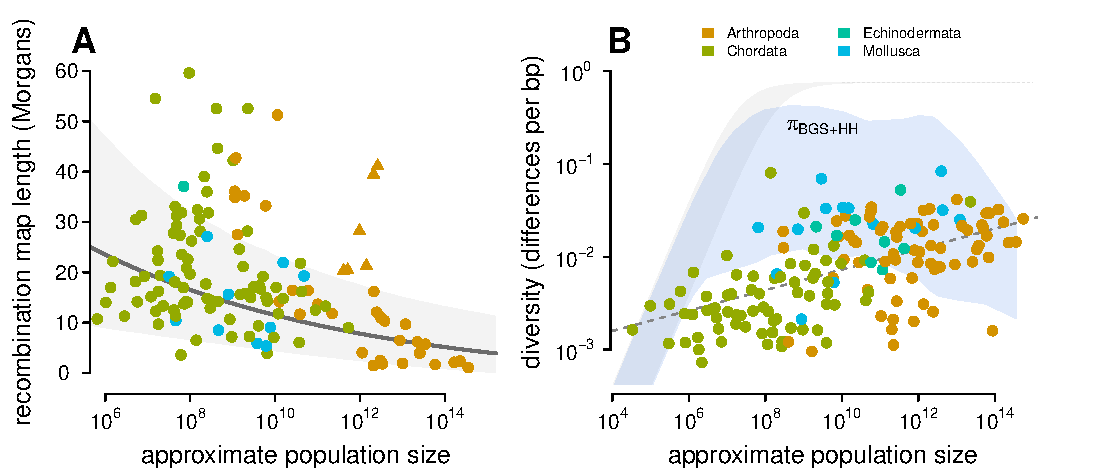
\includegraphics[width=\textwidth]{figures/figure_3.pdf}

  \caption{(A) The observed relationship between recombination map length ($L$)
    and census size ($N_c$) across 131 species with complete data and known
    phylogeny. Triangle points indicate social taxa excluded from the model
    fitting since these have adaptively higher recombination map lengths
    \parencite{Wilfert2007-dx}. The dark gray line is the estimated
    relationship under a phylogenetic mixed-effects model, and the gray
    interval is the 95\% posterior average.  (B) Points indicate the observed
    $\pi$--$N_c$ relationship across taxa shown in Figure \ref{fig:figure-1},
    and the blue ribbon is the range of predicted diversity were $N_e = N_c$
    for $\mu = 10^{-8}$--$10^{-9}$,  and after accounting for the expected
  reduction in diversity due to background selection and recurrent hitchhiking
under \emph{Drosophila melanogaster} parameters. In both plots, point color
indicates phylum.}

  \label{fig:figure-3}
\end{figure}

Previous work has found that the impact of linked selection increases with
$N_c$ (\cite{Corbett-Detig2015-gt}; see also Supplementary Figure
\ref{suppfig:corbett_detig}A), and it is often thought that this is driven by
higher rates of adaptive substitutions in larger populations, despite equivocal
evidence \parencite{Galtier2016-dq}. However, there is another mechanism by
which species with larger population sizes might experience a greater impact of
linked selection: recombinational map length, $L$, is known to correlate with
body mass \parencite{Burt1987-tq} and thus varies inversely with population
size. As this is a critical parameter that determines the genome-wide impact of
both hitchhiking and background selection, I examine the relationship between
recombination map length ($L$) and census population size ($N_c$) across taxa,
using available estimates of map lengths across species
\parencite{Stapley2017-fs,Corbett-Detig2015-gt}. I find a significant
non-linear relationship using phylogenetic mixed-effects models (Figure
\ref{fig:figure-3}A; see Methods: \Newnameref{sec:methods-pcm}). There is also
a correlation between map length and genome size (Supplementary Figure
\ref{supfig:genome_size_maplength}) and genome size and population size
(Supplementary Figure \ref{supfig:genome_size_popsize}). Overall, the negative
relationship between map length and census size indicates linked selection is
expected to be stronger in short map length, high-$N_c$ species.

Then, I predict the expected diversity ($\pi_{BGS+HH}$) under background
selection and hitchhiking, were $N_e= N_c$, and assuming all species had the
rate of sweeps and strength of BGS as \emph{D. melanogaster}. Since neutral
mutation rates $\mu$ are unknown and vary across species, I calculate the range
of predicted $\pi_{BGS+HH}$ estimates for $\mu = 10^{-8}$--$10^{-9}$ (using the
four-alleles model, \cite{Tajima1996-rb}), and compare this to the observed
relationship between $\pi$ and $N_c$ in Figured \ref{fig:figure-3}B.  Under
these parameters, linked selection begins to appreciably depress diversity
around $N_c \approx 10^9$, since $S \approx 10^{-8}$--$10^{-9}$ and linked
selection dominates drift when $S > \nicefrac{1}{2N}$.  Overall, this reveals
two problems for the hypothesis that linked selection could solve Lewontin's
Paradox. First, low to mid-$N_c$ species (census sizes between
$10^{6}$--$10^{14}$) have sufficiently long map lengths that their diversity
levels are only moderately reduced by linked selection, leading to a wide gap
between predicted and observed diversity levels. For this not to be the case,
the parameters that determine the strength of background selection and
recurrent hitchhiking would need to be \emph{higher} among these species than
in \emph{Drosophila melanogaster}. This would require that the rate of adaptive
mutations or the deleterious mutation rate be orders of magnitude higher for
species within this range than in \emph{Drosophila}, which is incompatible with
the rate of adaptive substitutions across species \parencite{Galtier2016-dq}
and mutation rates \parencite{Lynch2010-ki}. Furthermore, linked selection has
been quantified in humans, which fall in this census size range, and has been
found to be relatively weak
\parencite{McVicker2009-ax,Hernandez2011-gs,Hellmann2008-ic,Cai2009-by,Boyko2008-tj}.
Second, while hitchhiking and BGS can reduce predicted diversity levels for
high-$N_c$ species ($N_c > 10^{14}$) to observed levels, this would imply
available estimates of $\pi_0$ are underestimated by several orders of
magnitude in \emph{Drosophila} (Supplementary Figured
\ref{suppfig:corbett_detig}B). Overall, while linked selection could decouple
diversity from census size for high-$N_c$ species, recurrent hitchhiking and
background selection seem unlikely to explain the observed patterns of
diversity across species under our understanding of the range of parameter
estimates.

\section*{Discussion}

Nearly fifty years after Lewontin's description of the Paradox of Variation,
how evolutionary, life history, and ecological processes interact to constrain
diversity across taxa to a narrow range remains a mystery.  Since Wright
(\citeyear{Wright1931-fl,Wright1938-tv}), population geneticists have
appreciated that various demographic processes shrink effective population
sizes compared to census sizes, yet it has remained unclear whether these
neutral processes alone can explain Lewontin's Paradox and across-taxa
diversity patterns. Alternatively, selective processes that act more strongly
in larger populations could account for the observed narrow range of diversity.
A critical first step to discerning the processes that act to transform census
sizes to diversity levels across species is characterizing the observed
$\pi$--$N_c$ relationship.

Here, for 172 taxa, I estimated the relationship between genomic estimates of
pairwise diversity and approximate census population size. Previous surveys
have used allozyme-based estimates, fewer taxa, or qualitative measures of
population size. My estimates of census population sizes are quite approximate,
since they use body size to predict density. An improved estimate might
consider vagility (as \cite{Soule1976-he} did), though this is harder to do
systematically across many taxa. Future work might also use other ecological
information, such as total biomass and estimated numbers of species within
phyla, to improve census size estimates \parencite{Bar-On2018-kc, Mora2011-wm}.
Still, it seems more accurate estimates would be unlikely to change the
qualitative findings here, which resemble those of early surveys
\parencite{Nei1984-zi,Soule1976-he}.

One limitation of the dataset in this study is that diversity estimates are
collated from a variety of sources rather than estimated with a single
bioinformatic pipeline. This leads to technical noise across diversity
estimates; perhaps the relationship between $\pi$ and $N_c$ found here could be
tighter with a standardized bioinformatic pipeline. In addition to this
technical variation, there might be systematic bioinformatic sources of bias in
diversity estimates. For example high-diversity sequences may fail to align to
the reference genome and end up unaccounted for, leading to a downward bias.
Alternatively, high-diversity sequences might map to the reference genome, but
adjacent mis-matching SNPs might be mistaken for a short insertion or deletion.
While these issues might adversely affect the estimates in high-diversity
species, it is unlikely they will qualitatively change the observed
$\pi$--$N_c$ relationship.

\subsection*{Macroevolution and Across-Taxa Population Genomics}

% TODO -- talk about diversity as a trait. What are the trail evolution
% models?

Lewontin's Paradox arises from a comparison of diversity across species, yet
surprisingly, previous work on this problem has not considered the impact of
phylogenetic non-independence. I have addressed this limitation, showing that
diversity does have a significant positive relationship with census size, after
accounting for shared phylogenetic history among taxa. Additionally, I find a
high degree of phylogenetic signal, and that arthropods and chordates form
clusters, showing previous concern about phylogenetic non-independence was
warranted \parencite{Gillespie1991-qa}. Finally, this high degree of
phylogenetic signal, as well as evidence of shifts in the rate of evolution of
genetic diversity on deep timescales in molluscs and chordates, seem to
contradict Lynch's (2011) claim that since coalescent times are much less than
divergence times, they are not affected by shared phylogenetic history. 

One can reconcile my findings with Lynch's claim by considering what
evolutionary, ecological, life history, and demographic causal factors
determine coalescent rates across species, and how these factors evolve across
deep timescales. Lynch's conjecture that coalescent times should be free of
phylogenetic signal may be true \emph{were we to condition} on these causal
factors that could be affected by shared phylogenetic history. In contrast, my
estimates of phylogenetic signal in diversity are not conditioned on these
factors. Importantly, even ``correcting for" phylogeny implicitly favors
certain causal interpretations over others
\parencite{Westoby1995-wz,Uyeda2018-wf}. Future work could try to untangle what
causal factors determine coalescent times across species, as well as how these
factors evolve across macroevolutionary timescales.

Furthermore, beyond just accounting for phylogenetic non-independence,
macroevolution and phylogenetic comparative methods are a promising way to
approach across-species population genomic questions.  For example, one could
imagine that diversification processes could contribute to Lewontin's Paradox.
If large-$N_c$ species were to have a rate of speciation that is greater than
the rate at which mutation and drift reach equilibrium (which is indeed slower
for large $N_c$ species), this could act to decouple diversity from census
population size. That is to say, even if the rate of random demographic
bottlenecks were constant across taxa, lineage-specific diversification
processes could lead certain clades to be systematically further from
demographic equilibrium, and thus have lower diversity than expected for their
census population size. 

\subsection*{Spatial and Demographic Processes}

One limitation of this study is the inability to quantify the impact of spatial
population genetic processes on the relationship between diversity and census
population sizes across taxa. The genomic diversity estimates collated in this
study unfortunately lack details about the sampling process and spatial data,
which can have a profound impact on population genomic summary statistics
\parencite{Battey2020-lc}. These issues could systematically bias species-wide
diversity estimates; for example, if diversity estimates from a cosmopolitan
species were primarily from a single subpopulation, diversity would be an
underestimate relative to the entire population. However, biased spatial
sampling alone seems incapable of explaining the $\pi$-$N_c$ divergence in
high-$N_c$ taxa. In the extreme scenario in which only one subpopulation was
sampled, $F_\text{ST}$ would need to be close to one for population subdivision
alone to sufficiently reduce the total population heterozygosity to explain the
orders-of-magnitude shortfall between predicted and observed diversity levels.
This is because the equation for $F_{ST}$ can be rearranged such that $H_S =
(1-F_{ST})H_T$, where $H_S$ and $H_S$ are the subpopulation and total
population heterozygosities; if $H_T = 4N_c\mu$, then only $F_{ST} \approx 1$
can reduce $H_S$ several orders of magnitude. Yet, across-taxa surveys indicate
that $F_\text{ST}$ is almost never this high within species
\parencite{Roux2016-lm}.  Still, future work could quantify the extent to which
spatial processes contribute to Lewontin's Paradox. For example, high-$N_c$
taxa usually experience range expansions, likely with repeated founder effects
and local extinction/recolonization dynamics that doubtlessly depress
diversity. In particular, with the appropriate data, one could estimate the
empirical relationship between dispersal distance, range size, and coalescent
effective population size across taxa.

In this study, I have focused entirely on assessing the role of linked
selection, rather than demography, in reducing diversity across taxa. In
contrast to demographic models, models of linked selection have comparatively
fewer parameters and more readily permit rough estimates of diversity
reductions across taxa. Still, a full resolution of Lewontin's Paradox would
require understanding how the demographic processes across taxa with incredibly
heterogeneous ecologies and life histories transform $N_c$ into $N_e$. With
population genomic data becoming available for more species, this could involve
systematically inferring the demographic histories of tens of species and
looking for correlations in the frequency and size of bottlenecks with $N_c$
across species.

\subsection*{How could selection still explain Lewontin's Paradox?}

In this study, my goal was not to accurately estimate the levels in diversity
across species, but rather to give linked selection the best possible chance to
solve Lewontin's Paradox. Still, I find that even after parameterizing
hitchhiking and background selection with strong selection parameter estimates
from \emph{Drosophila melanogaster}, the predicted patterns of diversity under
linked selection poorly fit observed patterns of diversity across species.
While this suggests these two common modes of linked selection seem unlikely to
explain across-taxa patterns of diversity, there are three major potential
limitations of my approach that need further evaluation. 

First, I approximate the reduction in diversity using homogeneous background
selection and recurrent hitchhiking models
\parencite{Kaplan1989-sc,Hudson1995-xc,Coop2012-cd}, when in reality, there is
genome-wide heterogeneity in functional density, recombination rates, and the
adaptive substitutions across species. Each of these factors mediate how
strongly linked selection impacts diversity across the genome. Despite these
model simplifications, the predicted reduction in diversity in \emph{Drosophila
melanogaster} is $85\%$ (using $N_e$, not $N_c$), which is reasonably close to
the estimated $77\%$ from the more realistic model of Elyashiv et al. that
accounts for the actual position of substitutions, annotation features, and
recombination rate heterogeneity (though it should be noted that these both use
the same parameter estimates). Furthermore, even though my model fails to
capture the heterogeneity of functionality density and recombination rate in
real genomes, it is still extraordinary conservative, giving linked selection
the best possible chance to decouple diversity from census size and explain
Lewontin's Paradox. This is in part because the strong selection parameter
estimates from \emph{Drosophila melanogaster} used, but also because I assume
that the effective population size is the census size. Even then, this
decoupling only occurs in very high--census-size species, and implies that the
diversity in the absence of linked selection, $\pi_0$, is currently
underestimated by several orders of magnitude. Moreover, the study of
\textcite{Corbett-Detig2015-gt} did consider recombination rate and functional
density heterogeneity in estimating the reduction due to linked selection
across species, yet their predicted reductions are orders of magnitude weaker
than those considered here by assuming that $N_e = N_c$ (Supplementary Figure
\ref{suppfig:corbett_detig}B).  Overall, even with more realistic models of
linked selection, current models of linked selection seem fundamentally unable
to fit the diversity--census-size relationship.

Second, my model here only considers hard sweeps, and ignores the contribution
of soft sweeps (e.g. from standing variation or recurrent mutations;
\cite{Hermisson2005-hs,Pennings2006-lj}), partial sweeps (e.g those that do not
reach fixation), and the interaction of sweeps and spatial processes. While
future work exploring these alternative types of sweeps is needed, the
predicted reductions in diversity found here under the simplified sweep model
are likely relatively robust to these other modes of sweeps for a few reasons.
First, the shape of the diversity--recombination curve is equivalent under
models of partial sweeps and hard sweeps, though these imply different rates of
sweeps \parencite{Coop2012-cd}. Second, in the limit where most fitness
variation is due to weak soft sweeps from standing variation scattered across
the genome (i.e. due to polygenic fitness variation), levels of diversity are
well approximated by quantitative genetic linked selection models (QGLS
\cite{Robertson1961-ho,Santiago1995-hx,Santiago1998-bs}). The reduction in
diversity under these models is nearly identical to that under background
selection models, in part because deleterious alleles at mutation-selection
balance constitute a considerable component of fitness variation (see Appendix
Section \ref{app:bgs}; \cite{Charlesworth2000-km,Charlesworth2015-am}).
Finally, I also disregarded the interaction of sweeps and spatial processes.
For populations spread over wide ranges, limited dispersal slows the spread of
sweeps, allowing for new beneficial alleles to arise, spread, and compete
against other segregating beneficial variants
\parencite{Ralph2015-kl,Ralph2010-ki}. Through limited dispersal should act to
``soften sweeps" and not impact my findings for the reasons described above,
future work could investigate how these processes impact diversity in ways not
captured by hard sweep models.

Third, other selective processes, such as fluctuating selection or hard
selective events, could reduce diversity in ways not captured by the background
selection and hitchhiking model. Since frequency-independent fluctuating
selection generally reduces diversity under most conditions
\parencite{Novak2017-yp}, this could lead seasonality and other sources of
temporal heterogeneity to reduce diversity in large-$N_c$ species with short
generation times more than longer-lived species with smaller population sizes.
Future work could consider the impact of fluctuating selection on diversity
under simple models \parencite{Barton2000-zg} if estimates of key parameters
governing the rate of such fluctuations were known across taxa. Additionally,
another mode of selection that could severely reduce diversity across taxa, yet
remains unaccounted for in this study, is periodic hard selective events. These
selective events could occur regularly in a species' history yet be
indistinguishable from demographic bottlenecks from just population genomic
data. 

\subsection*{Measures of Effective Population Size, Timescales, and Lewontin's Paradox}

Lewontin's Paradox shows the extent to which the effective population sizes
implied by diversity, $\widetilde{N}_e$, diverge from census population sizes.
However, there are a variety other effective population size estimates
calculable from different data and summary statistics
\parencite{Wang2016-mi,Caballero1994-ao,Caballero2020-wm,Galtier2020-fb}. These
include estimators based on the observed decay in linkage disequilibrium or
temporal estimators that use the variance in allele frequency change. These
alternate estimators capture summaries of the effective population size on
shorter timescales than coalescent-based estimators \parencite{Wang2005-wy},
and thus could be used to tease out processes that impact the $N_e$-$N_c$
relationship in the more recent past. 

Temporal $N_e$ estimators already play an important role in understanding
another summary of the $N_e$-$N_c$ relationship: the ratio
$\nicefrac{N_e}{N_c}$, which is an important quantity in conservation genetics
\parencite{Frankham1995-xz,Mace1991-ai} and in understanding evolution in
highly-fecund marine species. Surveys of the $\nicefrac{N_e}{N_c}$ relationship
across taxa indicate mean $\nicefrac{N_e}{N_c}$ is on order of $\approx 0.1$
\parencite{Frankham1995-xz,Palstra2008-rt,Palstra2012-vy}, though the
uncertainty in these estimates is high, and some species with sweepstakes
reproduction systems like Pacific Oyster (\emph{Crassostrea gigas}) can have
$\nicefrac{N_e}{N_c} \approx 10^{-6}$. Estimates of the $\nicefrac{N_e}{N_c}$
ratio are an important, and under appreciated piece of solving Lewontin's
Paradox. For example, if $N_e$ is estimated from the allele frequency change
across a single generation (i.e. \cite{Waples1989-sj}), $\nicefrac{N_e}{N_c}$
constrains the variance in reproductive success
\parencite{Wright1938-tv,Nunney1993-ef,Nunney1996-wy}. This implies that apart
from species with sweepstakes reproductive systems, the variance in
reproductives success each generation (whether heritable or non-heritable) is
likely insufficient to significantly contribute to constraining
$\widetilde{N}_e$ for most taxa. Still, further work is needed to characterize
(1) how $\nicefrac{N_e}{N_c}$ varies with $N_c$ across taxa (though see
\cite{Palstra2012-vy}, Figure 2), and (2) the variance of $\nicefrac{N_e}{N_c}$
over longer time spans (i.e. how periodic sweepstakes reproductive events act
to constrain $N_e$). Overall, characterizing how $\nicefrac{N_e}{N_c}$ varies
across taxa and correlates with ecology and life history traits could provide
clues into the mechanisms that leads propagule size and survivorship curves to
be predictive of diversity levels across taxa
\parencite{Romiguier2014-bp,Hallatschek2018-iu,Barry2020-pp}.

Finally, short-term temporal $N_e$ estimators may play an important role in
resolving Lewontin's Paradox. These estimators, along with short-term estimates
of the impact of linked selection \parencite{Buffalo2019-qs,Buffalo2020-my},
can inform us how much diversity is depressed across shorter timescales, free
from the rare strong selective events or severe bottlenecks that impact
pairwise diversity. It could be that in any one generation, selection
contributes more to the variance of allele frequency changes than drift, yet
across-taxa patterns in diversity are better explained processes acting
sporadically on longer timescales, such as colonization, founder effects, and
bottlenecks. Thus, the pairwise diversity may not give us the best picture of
the generation to generation evolutionary processes acting in a population to
change allele frequencies. Furthermore, certain observed adaptations are
inexplicable given implied long-term coalescent effective population sizes, and
are only possible if short-term effective population sizes are orders of
magnitude larger \parencite{Karasov2010-fb,Barton2010-pi}.

\subsection*{Conclusions}

In \emph{Building a Science of Population Biology}
(\citeyear{Lewontin2004-fb}), Lewontin laments the difficulty of uniting
population genetics and population ecology into a cohesive discipline of
population biology. Lewontin's Paradox of Variation remains a critical unsolved
problem at the nexus of these two different disciplines: across species, we
fail to understand the processes that connect a central parameter of population
ecology, census size, to a central parameter of population genetics, effective
population size. Given that selection seems to fall short in explaining
Lewontin's Paradox, a full resolution will require a mechanistic understanding
the ecological, life history, and macroevolutionary processes that connect
$N_c$ to $N_e$ across taxa. While I have focused exclusively on metazoan taxa
since their population densities are more readily approximated from body mass,
a full resolution must also include plant species (with the added difficulties
of variation in selfing rates, different dispersal strategies, pollination,
etc.).

Looking at Lewontin's Paradox through an macroecological and macroevolutionary
lens begets interesting questions outside of the realm of population genetics.
Here, I have found that diversity and $N_c$ have a surprisingly consistent
relationship without many outliers, despite the wildly disparate ecologies,
life histories, and evolutionary histories of the taxa included. Furthermore,
taxa with very large census sizes have surprisingly low diversity. Is this
explained by macroevolutionary processes, such as different rates of speciation
for large-$N_c$ taxa? Or, are the levels of diversity we observe today an
artifact of our timing relative to the last glacial maximum, or the last major
extinction? Did large-$N_c$ prehistoric animal populations living in other
geological eras have higher levels of diversity than our present taxa? Or, does
ecological competition occur on shorter timescales such that strong population
size contractions transpire and depress diversity, even if a species is
undisturbed by climatic shifts or mass extinctions? Overall, patterns of
diversity across taxa are determined by many overlaid evolutionary and
ecological processes occurring on vastly different timescales. Lewontin's
Paradox of Variation may persist unresolved for some time because the solution
requires synthesis and model building at the intersection of all these
disciplines.


\section*{Methods}

\subsection*{Diversity and Map Length Data}
\label{sec:methods-diversity}

The data used in this study are collated from a variety of previously published
surveys. Of the 172 taxa with diversity estimates, 14 are from
\textcite{Corbett-Detig2015-gt}, 96 are from \textcite{Leffler2012-zj}, and 62
are from \textcite{Romiguier2014-bp}. The Corbett-Detig et al. data is
estimated from four-fold degenerate sites, the Romiguier et al. data is
synonymous sites, and the Leffler et al. data is estimated predominantly from
silent, intronic, and non-coding sites. All types of diversity estimates from
\textcite{Leffler2012-zj} were included to maximize the taxa in the study,
since the variability of diversity across functional categories is much less
than the diversity across taxa. Multiple diversity estimates per taxa were
averaged. The total recombination map length data were from both
\citeauthor{Stapley2017-fs} (2017; 30 taxa), and
\citeauthor{Corbett-Detig2015-gt} (2015; 11 taxa). Both studies used
sex-averaged recombination maps estimated with cross-based approaches; in some
cases errors in the original data were found, documented, and corrected. These
studies also included genome size estimates used to create Supplementary
Figures \ref{supfig:genome_size_popsize} and
\ref{supfig:genome_size_maplength}. 

\subsection*{Macroecological Estimates of Population Size}
\label{sec:methods-popsize}

A rough approximation for total population size (census size) is $N_c = D R$,
where $D$ is the population density in individuals per $\text{km}^2$ and $R$ is
the range size in $\text{km}^2$. Since population density estimates are not
available for many taxa included in this study, I used the macroecological
abundance-body size relationship to predict population density from body size.
Since body length measurements are more readily available than body mass, I
collated body length data from various sources (see
\url{https://github.com/vsbuffalo/paradox_variation/}); body lengths were
averaged across sexes for sexually dimorphic species, and if only a range of
lengths was available, the midpoint was used.

Then, I re-estimated the relationship between body mass and population density
using the data in the appendix table of \textcite{Damuth1987-sg}, which
includes 696 taxa with body mass and population density measurements across
mammals, fish, reptiles, amphibians, aquatic invertebrates, and terrestrial
arthropods. Though the abundance-body size relationship can be noisy at small
spatial or phylogenetic scales \parencite[Chapter 5,][]{Gaston2008-pn}, across
deeply diverged taxa such as those included in this study and
\textcite{Damuth1987-sg}, the relationship is linear and homoscedastic (see
Supplementary Figure \ref{suppfig:damuth}). Using Stan
\parencite{Stan_Development_Team2020-ea}, I jointly estimated the relationship
between body mass from body length using the \textcite{Romiguier2014-bp} taxa,
and used this relationship to predict body mass for the taxa in this study.
These body masses were then used to predict population density simultaneously,
using the \textcite{Damuth1981-st} relationship. The code of this routine
(\texttt{pred\_popsize\_missing\_centered.stan}) is available in the GitHub
repository (\url{https://github.com/vsbuffalo/paradox_variation/}).

To estimate range, I first downloaded occurrence records from Global
Biodiversity Information Facility \parencite{noauthor_2020-ey} using the
\texttt{rgbif} R package \parencite{Chamberlain2014-up,Chamberlain2017-uz}.
Using the occurrence locations, I inferred whether a species was marine or
terrestrial, based on whether the majority of their recorded occurrences
overlapped a continent using \texttt{rnaturalearth} and the \texttt{sf}
packages \parencite{South2017-db,Pebesma2018-bs}. For each taxon, I estimated
its range by finding the minimum $\alpha$-shape containing these occurrences.
The $\alpha$ parameters were set more permissive for marine species since
occurrence data for marine taxa were sparser. Then, I intersected the inferred
ranges for terrestrial taxa with continental polygons, so their ranges did not
overrun landmasses (and likewise with marine taxa and oceans). I inspected
diagnostic plots for each taxa for quality control (all of these plots are
available in \texttt{paradox\_variation} GitHub repository), and in some cases,
I manually adjusted the $\alpha$ parameter or manually corrected the range
based on known range maps (these changes are documented in the code
\texttt{data/species\_ranges.r} and \texttt{data/species\_range\_fixes.r}).
The range of \emph{C. elegans} was conservatively approximated as the area of
the Western US and Western Europe based on the map in \textcite{Frezal2015-iw}.
\emph{Drosophila} species ranges are from the Drosophila Speciation Patterns
website, \parencite{Yukilevich2012-vn,Yukilevich2017-jg}. To further validate
these range estimates, I have compared these to the qualitative range
descriptions \textcite{Leffler2012-zj} (Supplementary Figure
\ref{suppfig:range-cats}) and compared my $\alpha$-shape method to a subset of
taxa with range estimates from IUCN Red List
(\cite{Chamberlain2020-tv,Iucn2020-ap}; Supplementary Figure
\ref{suppfig:redlist-ranges}). Each census population size is then estimated as
the product of range and density. 

\subsection*{Phylogenetic Comparative Methods}
\label{sec:methods-pcm}

Of the full dataset of 172 taxa with diversity and population size estimates, a
synthetic calibrated phylogeny was created for 166 species that appear in
phylogenies in DateLife project \parencite{OMeara2020-ds,Sanchez-Reyes2019-io}.
This calibrated synthetic phylogeny was then subset for the analyses based on
what species had non-missing trait data. The diversity-population size
relationship assessed by a linear phylogenetic mixed-effects model implemented
in Stan \parencite{Stan_Development_Team2020-ea}, according to the methods
described in (\cite{De_Villemereuil2014-kt}, see
\texttt{stan/phylo\_mm\_regression.stan} in the GitHub repository). This same
Stan model was used to estimate the same relationship between arthropod,
chordate, and mollusc subsets of the data (Supplementary Figure
\ref{suppfig:div_popsize_post_phyla}). 

The relationship between recombination map length and the logarithm of
population size is non-linear and heteroscedastic, and was fit using a
lognormal phylogenetic mixed-effects model. Since social insects have longer
recombination map lengths \parencite{Wilfert2007-dx}, social taxa were excluded
when fitting this model.  All \texttt{Rhat} \parencite{Vehtari2019-po} values
were below 1.01 and the effective number of samples was over 1,000, consistent
with good mixing; details about the model are available in the GitHub
repository (\texttt{phylo\_mm\_lognormal.stan}). Continuous trait maps (Figure
\ref{fig:figure-2}A and Supplementary Material Figure \ref{suppfig:biconmap})
were created using \texttt{phytools} \parencite{Revell2012-zq}. Node-height
tests were implemented based on the methods in \texttt{Geiger}
\parencite{Pennell2014-nx,Harmon2008-tr}, and use robust regression to fit a
linear relationship between phylogenetic independent contrasts and branching
times.

\subsection*{Predicted Reductions in Diversity}
\label{sec:methods-reduction}

The predicted reductions in diversity due to linked selection are approximated
using selection and deleterious mutation parameters from \emph{Drosophila
melanogaster}, and the recombination map length estimates from
\textcite{Stapley2017-fs} and \textcite{Corbett-Detig2015-gt}. The mathematical
details of the simplified sweep model are explained in the Appendix Section
\ref{app:sweep}. I use estimates of the number of substitutions, $m$, in genic
regions between \emph{D.  melanogaster} and \emph{D. simulans} from
\textcite{Hu2013-pg}.  Following \textcite{Elyashiv2016-vt}, only substitutions
in UTRs and exons are included, since they found no evidence of sweeps in
introns. Then, I average over annotation classes to estimate the mean
proportion of substitutions that are beneficial, $\alpha_\text{Dmel}=0.42$,
which are consistent with the estimates of Elyashiv et al. and estimates from
MacDonald--Kreitman test approaches (see \cite{Eyre-Walker2006-li}, Table 1).
Then, I use divergence time estimates between \emph{D. melanogaster} and
\emph{D. simulans} of $4.2 \times 10^6$ and estimate of ten generations per
year \parencite{Obbard2012-on}, calculating there are $\gamma_\text{Dmel} =
\nicefrac{\alpha m}{2T} = 2.26 \times 10^{-3}$ substitutions per generation.
Given the length of the \emph{Drosophila} autosomes, $G$, this implies that the
rate of beneficial substitutions per basepair, per generation is $\nu_{BP,Dmel}
= \nicefrac{\gamma_\text{Dmel}}{G} = 2.34 \times 10^{-11}$. Finally, I estimate
$J_\text{Dmel}$ from the estimate of genome-wide average rate of sweeps from
Elyashiv et al. (Supplementary Table S6) and assuming \emph{Drosophila} $N_e =
10^6$. These \emph{Drosophila melanogaster} hitchhiking parameter estimates are
close to other previously-published estimates (Supplementary Figure
\ref{suppfig:linked-sel-params}). Finally, I use $U_\text{Dmel} = 1.6$, from
\textcite{Elyashiv2016-vt}. With these parameter estimates from \emph{D.
melanogaster}, the recombination map lengths across species, and Equation
\eqref{eqn:div}, I estimate $\pi_\text{BGS+HH}$ (assuming $N_c=N_c$) across all
species. This leads to a range of predicted diversity ranges across species
corresponding to $\mu=10^{-8}$--$10^{-9}$; to visualize these, I take a convex
hull of all diversity ranges and smooth this with R's \texttt{smooth.spline}
function.



\section*{Acknowledgments}

I would like to thank Andy Kern and Peter Ralph for helpful discussions and
supporting me during this work, and Graham Coop for inspiration and helpful
feedback during socially distanced nature walks at Yolo Basin. I thank Jessica
Stapley for kindly providing the recombination map length data, and Yaniv
Brandvain, Amy Collins, Doc Edge, Tyler Kent, Chuck Langley, Matt Osmond, Sally
Otto, Jeff Ross-Ibarra, Aaron Stern, Anastasia Teterina, Michael Turelli,
Margot Wood, and my Kern-Ralph labmates for helpful discussions. Sarah
Friedman, Katherine Corn, and Josef Uyeda provided very useful advice about
phylogenetic comparative methods; yet I take full responsibility for any
shortcomings of my analysis.  I would like to also thank UO librarian Dean
Walton for helping me track down some rather difficult to find older papers.
This work was supported by an NIH Grant (1R01GM117241) awarded to Andrew Kern.

\section*{Appendix}

\setcounter{table}{0}
\renewcommand{\theequation}{A\arabic{equation}}
\setcounter{section}{0}
\renewcommand{\thesection}{A\arabic{section}}
\setcounter{figure}{0}
\renewcommand{\thefigure}{A\arabic{figure}}


\section{Simplified Sweep Effects Model}
\label{app:sweep}

I use a simplified model of the effects of recurrent hitchhiking and background
selection (BGS) occurring uniformly along a genome. Expected diversity is given
by

\begin{align}
  \E(\pi) &= \frac{\theta}{\theta + \nicefrac{1}{B} + 2NS} \\
          &\approx \frac{\theta}{\nicefrac{1}{B} + 2NS} 
\end{align}
%
(cf. equation 1 \cite{Elyashiv2016-vt}, and equation 20 of \cite{Coop2012-cd}).
The BGS component is given by \textcite{Hudson1995-xc},

\begin{align}
  B(U, L) = N_e \exp\left(-\frac{U}{L}\right)
\end{align}
%
and the hitchhiking component is

\begin{align}
  S = \frac{\nu_\text{BP}}{r_\text{BP}} J
\end{align}
%
(cf. \cite{Coop2012-cd} equation 20) where $J$ is the probability that two
lineages coalesce down to one, given sweeps occur uniformly along the genome.
Under this homogeneous sweep model, $J$ is 

\begin{align}
  J = \int_0^L q_f(r)^2 dr 
\end{align}
%
where $q_f(r)$ is the approximate probability that a lineage is trapped by a
sweep to frequency $f$ when it is $r$ recombination fraction away from this
sweep (cf. \cite{Coop2012-cd} equation 15). 

Since I use \emph{Drosophila melanogaster} parameter estimates from
\textcite{Elyashiv2016-vt}, I now reconcile their model's $S$ term with the
simple model above. They estimate $S$ in \emph{Drosophila melanogaster} using a
composite likelihood model that considers hitchhiking and background selection
simultaneously, using substitutions and stratifying by annotation.  For a
neutral position at site $x$, the coalescent rate due to sweeps is given by
Elyashiv et al.'s equation 3, 

\begin{align}
  S(x) = \frac{1}{T} \sum_{i_S} \alpha(i_S) \sum_{y \in a(i_S)} \int \exp(-r(x, y) \tau(s, N)) g(s | i_S) ds
\end{align}
%
where $T$ is the number of generations that substitutions accrue, $i_S = 1,
\ldots, I_S$ is the annotation class (e.g. exons, introns, UTRs), $\alpha(i_S)$
is the fraction of substitutions in annotation class $i_S$ that are beneficial,
$a(i_S)$ is the set of all substitutions in annotation class $i_S$, $\tau(s,
N)$ is the fixation time of a site with additive effect $s$, and $g(s | i_S)$
is the distribution of selection coefficients for annotation class $i_S$. 

Note, that we can recover the model of \textcite{Coop2012-cd} from this
expression. Suppose there is only one annotation class, and $\alpha$ fraction
of substitutions are beneficial, and one selection coefficient $\bar{s}$, (i.e.
$g(s) = \delta_0(s - \bar{s})$), then

\begin{align}
  S(x) = \frac{\alpha}{T} \sum_{y \in {a}} \exp(-r(x,y)\tau(\bar{s}, N)).
\end{align}
%

Let the number of substitutions be $m := |a|$, and imagine their positions are
uniformly distributed on a segment of length $G$ basepairs with the focal site
is the middle at position $x=0$. Then, each substitution $y$ is a random
distance $l_y \sim U(-\nicefrac{G}{2}, \nicefrac{G}{2})$ away from the focal
site. Assuming the recombination rate is a constant $r_\text{BP}$ per
basepair, and approximating the sum with an integral, we have,

\begin{align}
  S &= \frac{\alpha}{T} \sum_{i=1}^m \E_{l_i} \left(\exp(-r_\text{BP} l_i \tau(\bar{s}, N)) \right) \\
    &= \frac{\alpha}{T G} \sum_{i=1}^m \int_0^{G} \exp(-r_\text{BP} \ell \tau(\bar{s}, N)) d\ell \\
    &= \frac{\alpha m}{T G} \int_0^{G} \exp(-r_\text{BP} \ell \tau(\bar{s}, N)) d\ell
\end{align}

Using $u$-substitution with $r = \ell r_\text{BP}$ this simplifies to

\begin{align}
  S &= \frac{\alpha m}{T G r_\text{BP}} \int_0^{L} \exp(-r \tau(\bar{s}, N)) dr
\end{align}
%
where $L = G r_\text{BP}$. 

To simplify this notation, note that the rate of adaptive substitutions per
basepair per generation is $\nu_\text{BP} = \nicefrac{\alpha m}{GT}$, so 

\begin{align}
  S &= \frac{\nu_\text{BP}}{r_\text{BP}} \int_0^{L} \exp(-r \tau(\bar{s}, N)) dr
\end{align}

This is analogous to the second term of \textcite{Coop2012-cd} equation 17,
with $k = i = 2$ and $x = 1$ (e.g.  conditioning on a sweep to fixation). Note
that there appears to be a factor of two error in \textcite{Elyashiv2016-vt}
compared to \textcite{Coop2012-cd}; here I include the factor of two.  Then,

\begin{align}
  S &= \frac{\nu_\text{BP}}{r_\text{BP}} \underbrace{\int_0^{L} \exp(-2r \tau(\bar{s}, N)) dr}_{J}
\end{align}
%

where the integral is equal to $J$ (c.f. $J_{2,2}$ of equation 15 in
\cite{Coop2012-cd}) since a simple model of $q_f(r) = f \exp(- 2r \tau(s, N))$
and if we condition on fixation, $f = 1$. This expression is useful to
generalize across species, since we know $N$ and $L$. Additionally, we have
estimates of $\alpha$ and $\nicefrac{m}{T}$ in \emph{Drosophila} and other
species. In Elyashiv et al, they consider the number of substitutions per
generation in genic regions only; it should be noted that the number of coding
basepairs varies little across species. For convenience, I define $\gamma =
\nicefrac{\alpha m}{T}$ as the number of adaptive substitutions per generation
per entire genome, such that $S(\gamma, L, J) = \nicefrac{\gamma}{L} \; J$ used
in the main text. Using the estimates of $m \approx 4.5 \times 10^{5}$, $\alpha
\approx 0.42$, and $T \approx 8.4 \times 10^{7}$ from the Supplementary
Material of Elyashiv et al., I arrive at $\gamma \approx 0.00226$ adaptive
substitutions per generation, per genome. For a $\approx 100$ megabase genome,
this translates to a $\nu_\text{BP} \approx 2.34 \times 10^{-11}$, which is
close to previous estimates (Supplementary Figure
\ref{suppfig:linked-sel-params}). For $J$, I use an empirical estimate
calculated from the genome-wide average of the rate of coalescent events due to
sweeps, from Supplementary Table S6 of Elyashiv et al. ($r_s = 2NS \approx
0.92$). This implies $J \approx 4.46 \times 10^{-4}$. Alternatively, I have
tried using the estimated distribution of selection coefficients from Elyashiv
et al., but this led to a weaker estimate of $J$, since the adaptive
substitutions considered tend to cluster around genic regions. Note that these
\emph{Drosophila} sweep parameters I have used are close to previous estimates
(Supplementary Figures \ref{suppfig:linked-sel-params} A and B). 

%Given that \textcite{Elyashiv2016-vt} provides a distribution of binned
%selection coefficients $g(s|i_S)$ by annotation class $i_S$ (e.g. UTRs, exons),
%I average over $i_S$, weighting by the number of basepairs in each annotation
%category, to calculate the marginal distribution of selection coefficients $g(s)$. 
%Then, I calculate $J$ by marginalizing over $g(s)$, 

%\begin{align}
%  J = \sum_{s} g(s) \int_{0}^{L} \exp(- 2 r \tau(s, N)) dr.
%\end{align}
%%
%Throughout, I use the expression for fixation time, 

%\begin{align}
%  \tau(s, N) = \frac{2}{s} \left(\log(4 N s) + c - \nicefrac{1}{4Ns}\right)
%\end{align}
%%
%from equation A17 of \textcite{Hermisson2005-hs}, re-parameterized so the
%fitness of the heterozygote is $1+s$, and $c \approx 0.577$ is Euler's gamma.

%% We can take $L \to \infty$ as
%% in \textcite{Coop2012-cd}, leaving

%% \begin{align}
%%   S &= \frac{\alpha m}{T} \frac{1}{L \tau(\bar{s}, N)} 
%% \end{align}

\section{Background Selection and Polygenic Fitness Models}
\label{app:bgs}

Throughout the main text, I use recurrent hitchhiking and background selection
models to estimate the reduction in diversity due to linked selection. Another
class of linked selection models, which I refer to as quantitative genetic
linked selection models (QGLS;
\cite{Robertson1961-ho,Santiago1995-hx,Santiago1998-bs}), can also depress
genome-wide diversity. Furthermore, these models may depress diversity at neutral sites unlinked to the regions containing fitness variation.  While I
did not explicitly incorporate these models into my estimates of the diversity
reductions, their effect is implicit in background selection models because
they are analytically nearly identical. Here, I briefly sketch out the
connection between BGS and QGLS models.

Under the \textcite{Santiago1998-bs} model, the effective population size is
$N_e^\text{SC98} = N \exp(\nicefrac{-C^2}{(1-Z)L})$, where $C^2$ is the
standardized heritable fitness variation, $1-Z$ is the decay of genetic
variance through time, and $L$ is the recombination map length. This model can
accommodate a variety of modes of selection such as selection on an
infinitesimal trait \parencite[p.  1016]{Santiago1995-hx}, and the flux of
either weakly advantageous or deleterious alleles \parencite[p.
2109]{Santiago1998-bs}. If the source of fitness variation is entirely the
input of new deleterious mutations with heterozygous effect $s h$ at rate $U$
per diploid genome per generation, then under mutation-selection balance, the
equilibrium relative variance in reproductive success $C^2 = U sh$
(\cite{Crow1970-wm}; \cite{Caballero2020-wm}, p. 167), and $Z = 1 - sh -
\nicefrac{1}{2N_c}$ \parencite{Santiago1998-bs}. Thus, if $\nicefrac{1}{2N_c}
<< sh << 1$, then $\nicefrac{C^2}{(1-Z)} \approx U$ and $N_e^\text{SC98}
\approx N \exp(\nicefrac{-U}{L})$, which is the BGS model used in the main text
and is a result of many background selection models with similar assumptions
(\cite{Hudson1994-oh} eqn.  15; \cite{Hudson1995-xc} eqn.  9;
\cite{Nordborg1996-nq} eqn. 4; \cite{Barton1995-pm} eqn. 22b). Intuitively, the
similarity of these models reflects the fact that a substantial proportion of
heritable fitness variation is caused by the continual flux of deleterious
alleles across the genome under mutation-selection balance
\parencite{Charlesworth2015-am,Charlesworth2000-km}. 


\printbibliography

\setcounter{table}{0}
\renewcommand{\thetable}{S\arabic{table}}
\setcounter{equation}{0}
\renewcommand{\theequation}{S\arabic{equation}}
\setcounter{section}{0}
\renewcommand{\thesection}{S\arabic{section}}
\setcounter{figure}{0}
\renewcommand{\thefigure}{S\arabic{figure}}

\section*{Supplementary Information}

\section{Population Size Validation}

The approximate census sizes I have estimated here


\begin{figure}[!htb]
  \centering
  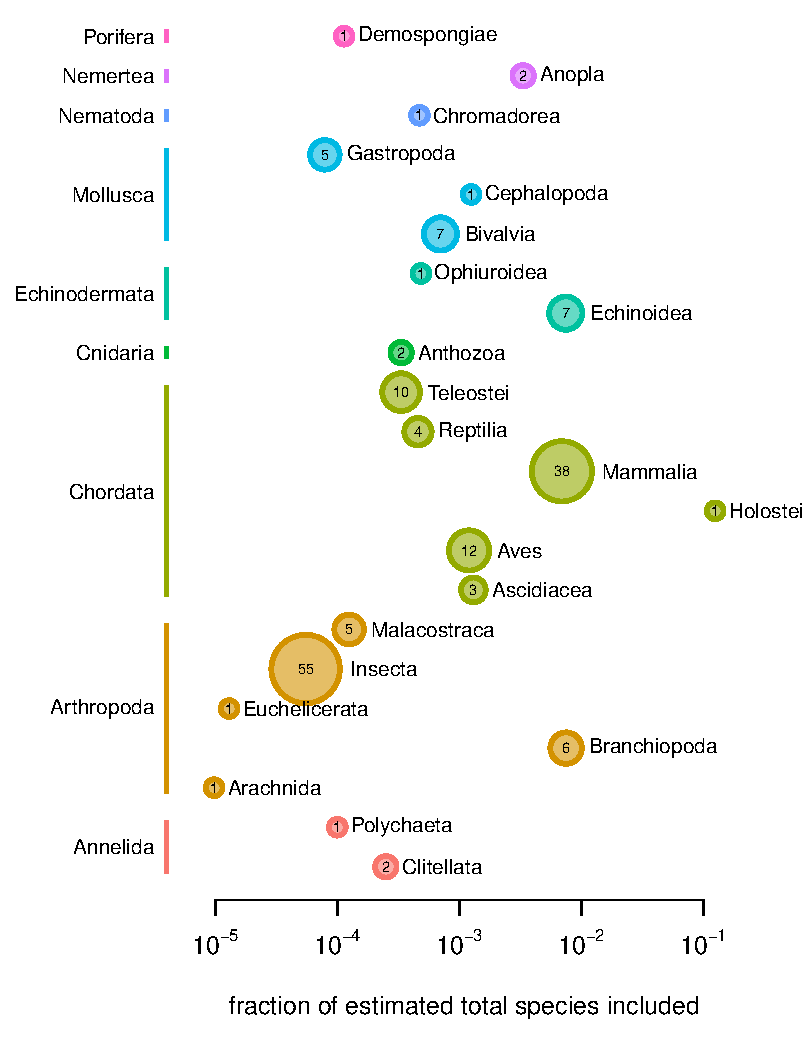
\includegraphics[]{figures/species_counts.pdf}

  \caption{}

  \label{suppfig:species_counts}
\end{figure}

\begin{table}[ht]
  \resizebox{\textwidth}{!}{%
\centering
\begin{tabular}{lr|rr|rrrr|r}
  &  & \multicolumn{2}{c}{\bf Bar-On et al.}  & \multicolumn{4}{c}{\bf Present study}  &  \\
  phylum & total species ($T$) & biomass ($B$) & prop. biomass & biomass ($b$) &  prop. biomass & num. species ($n$) &prop. total species ($f = \nicefrac{n}{T}$) & factor ($\nicefrac{b}{f B}$) \\
  \hline
  Arthropoda & $1.26 \times 10^{6}$ & 1.20 & 0.4635 & $2.77 \times 10^{-4}$ & 0.0100 &  68 & $5.41 \times 10^{-5}$ & 4.26 \\
  Chordata & $5.41 \times 10^{4}$ & 0.87 & 0.3357 & $2.68 \times 10^{-2}$ & 0.9720 &  68 & $1.26 \times 10^{-3}$ & 24.50 \\
  Annelida & $1.70 \times 10^{4}$ & 0.20 & 0.0772 & $1.24 \times 10^{-5}$ & 0.0005 &   3 & $1.76 \times 10^{-4}$ & 0.35 \\
  Mollusca & $9.54 \times 10^{4}$ & 0.20 & 0.0772 & $4.47 \times 10^{-4}$ & 0.0162 &  13 & $1.36 \times 10^{-4}$ & 16.40 \\
  Cnidaria & $1.60 \times 10^{4}$ & 0.10 & 0.0386 & $3.21 \times 10^{-5}$ & 0.0012 &   2 & $1.25 \times 10^{-4}$ & 2.57 \\
  Nematoda & $2.50 \times 10^{4}$ & 0.02 & 0.0077 & $4.00 \times 10^{-6}$ & 0.0001 &   1 & $4.00 \times 10^{-5}$ & 5.00 \\
\end{tabular}}

  \caption{How the total carbon biomass estimates by phylum from
    \textcite{Bar-On2018-kc} compare to the implied biomass estimates from this
    study. All biomass estimates are carbon biomass, and the proportions are of
    total biomass with respect to the study. The proportion of biomass in this
    study compared to the Bar-On et al. estimates \textcite{Bar-On2018-kc}
    indicates chordates are over-represented and arthropods are
    under-represented in the present study. Total species by phylum estimates
  are from
\textcite{Reaka-Kudla1996-fe,Nicol1969-qx,Zhang2013-zc,Chapman2009-fw}. The
ratio column is the ratio of total biomass implied by the $N_c$ estimates of
each species in a phylum to the actual biomass of that phylum.}

\end{table}




\section{Diversity and IUCN Red List Status}
\label{supinfo:div-iucn}

I also investigated the relationship between species' IUCN Red List categories
(an ordinal scale of how threatened a species is) and both diversity and
population size, finding that species categorized as more threatened have both
smaller population sizes and reduced diversity, compared to non-threatened
species (Supplementary Figure \ref{suppfig:figure-1-redlist}) consistent with
past work \parencite{Spielman2004-mt}. A linear model of diversity regressed on
population size has lower AIC when the IUCN Red List categories are included,
and the estimates of the effect of IUCN status are all negative on diversity,
though not all are significant in part because some categories have three or
fewer species (Supplementary Table \ref{supptable:tbl-1}).

\begin{figure}[t!]
  \centering
  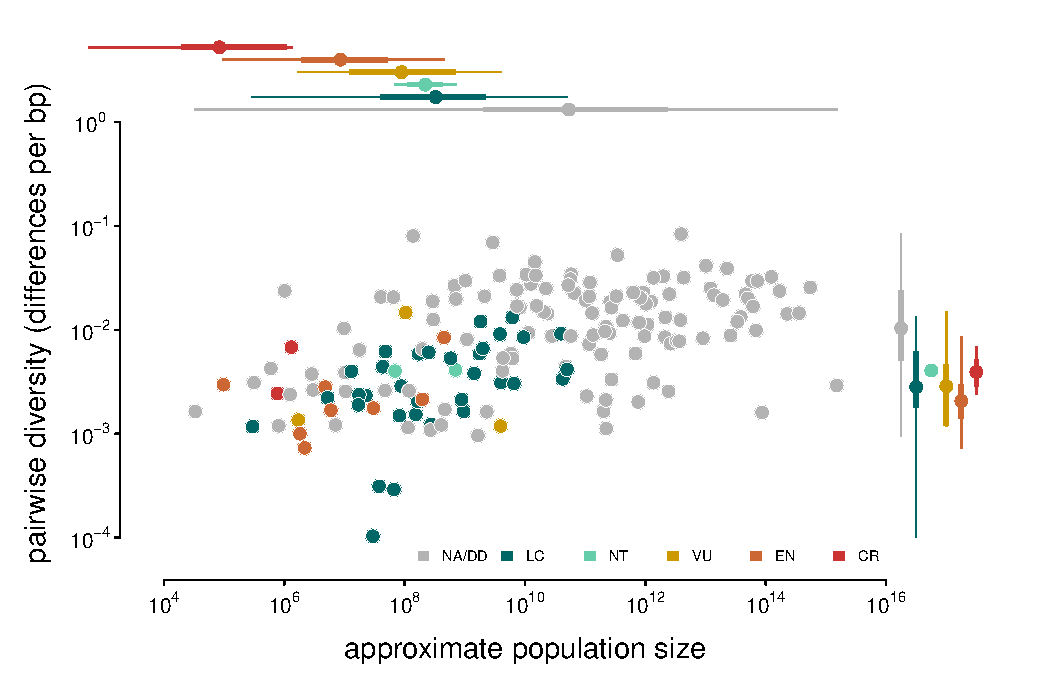
\includegraphics[width=\textwidth]{figures/diversity_popsize_redlist.pdf}

  \caption{A version of Figure \ref{fig:figure-1} with points colored by their
    IUCN Red List conservation status. Margin boxplots show the diversity and
    population size ranges (thin lines) and interquartile ranges (thick lines)
    for each category. NA/DD indicates no IUCN Red List entry, or Red List
  status Data Deficient; LC is Least Concern, NT is Near Threatened, VU is
Vulnerable, EN is Endangered, and CR is Critically Endangered.}

  \label{suppfig:figure-1-redlist}
\end{figure}



\begin{table}[ht]
  \centering
  \begin{tabular}{rrrr}
    \hline
 & mean & 2.5 \% & 97.5 \% \\ 
 \hline
    $\beta_0$ & -2.70 & -3.00 & -2.40 \\ 
    $\beta_{LC}$ & -0.37 & -0.55 & -0.19 \\ 
    $\beta_{NT}$ & -0.19 & -0.80 & 0.41 \\ 
    $\beta_{VU}$ & -0.31 & -0.81 & 0.19 \\ 
    $\beta_{EN}$ & -0.39 & -0.71 & -0.06 \\ 
    $\beta_{CR}$ & -0.03 & -0.65 & 0.59 \\ 
    $\beta_{N_c}$ & 0.06 & 0.04 & 0.09 \\ 
    \hline
  \end{tabular}

  \caption{The regression estimates of full IUCN Red List population size model
    for diversity, $\log_{10}(\pi) = \beta_0 + \beta_{LC} LC + \beta_{NT} NT +
    \beta_{VU} VU + \beta_{EN} EN + \beta_{CR} CR + \beta_{N_c} \log_{10}(N_c)$;
    $df = 165$.  Using AIC to compare this full model to a reduced model of
    $\log_{10}(\pi) = \beta_0 + \beta_{N_c} \log_{10}(N_c)$, $AIC_\text{full} =
  203.99$, $AIC_\text{reduced} =212.46$. }

\end{table}
\label{supptable:tbl-1} 
\begin{figure}[!htb]
  \centering
  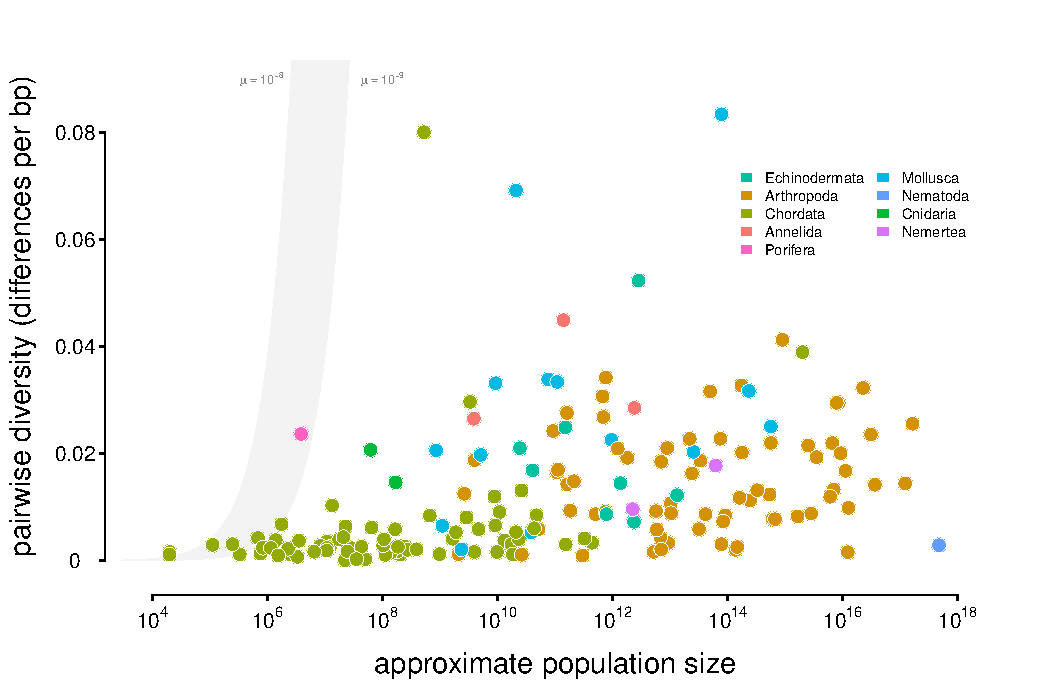
\includegraphics[width=\textwidth]{figures/diversity_popsize_linear.pdf}

  \caption{A version of Figure \ref{fig:figure-1} with diversity on a linear,
    rather than log, scale. Points are colored by phylum, and the shaded region
    is the predicted neutral level of diversity assuming $N_e = N_c$ with mutation
  range ranging between $10^{-10} \le \mu \le 10^{-8}$. }

  \label{suppfig:figure-1-linear}
\end{figure}

\begin{figure}[!htb]
  \centering
  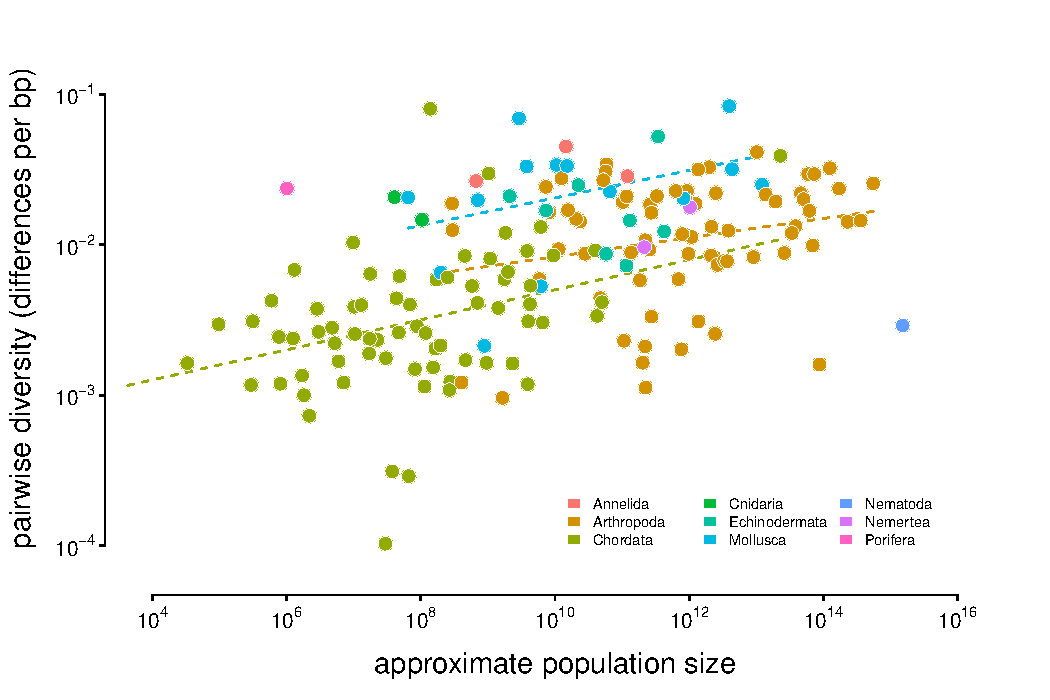
\includegraphics[width=\textwidth]{figures/diversity_popsize_averages.pdf}

  \caption{Diversity and approximate population size for 172 taxa, colored by
    phylum; the dashed lines indicate the non-phylogenetic OLS estimates of the
  relationship between population size and diversity grouped by phyla.}

  \label{suppfig:figure-1-ave}
\end{figure}


\begin{figure}[!htb] \centering
  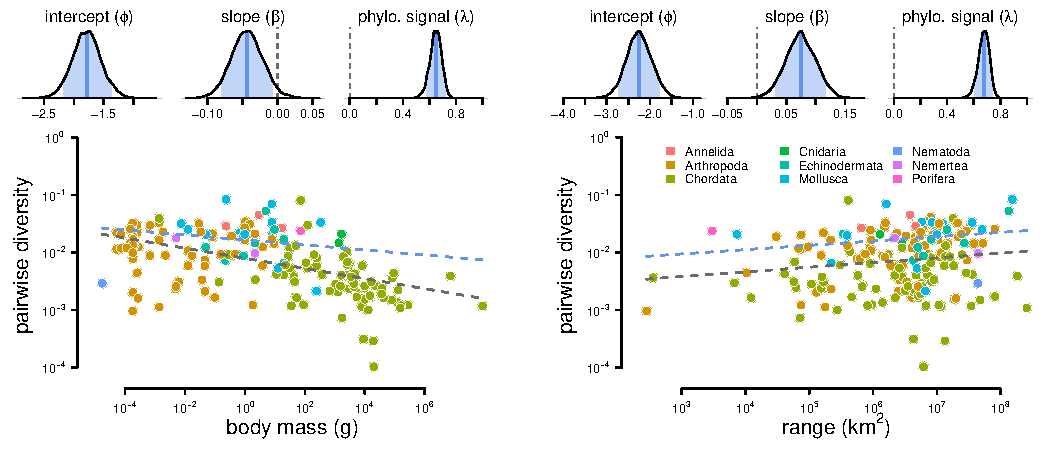
\includegraphics[width=\textwidth]{figures/diversity_range_bodymass.pdf}

  \caption{The relationship between diversity (differences per basepair) and
    body mass (left) and range (right) across 172 species. The top row are
    posterior distributions of parameters estimated using the phylogenetic
    mixed-effects model using 166 taxa in the synthetic phylogeny for the
    intercept, slope, and phylogenetic signal from the mixed-effects model. The
    bottom row contain each species as a point, colored by phyla. The gray
    dashed line is the non-phylogenetic standard regression estimate, and the
    blue dashed line is the relationship fit by the phylogenetic mixed-effects
  model. }

  \label{suppfig:figure-div-range-bodymass}
\end{figure}



\begin{figure}[!htb]
  \centering
  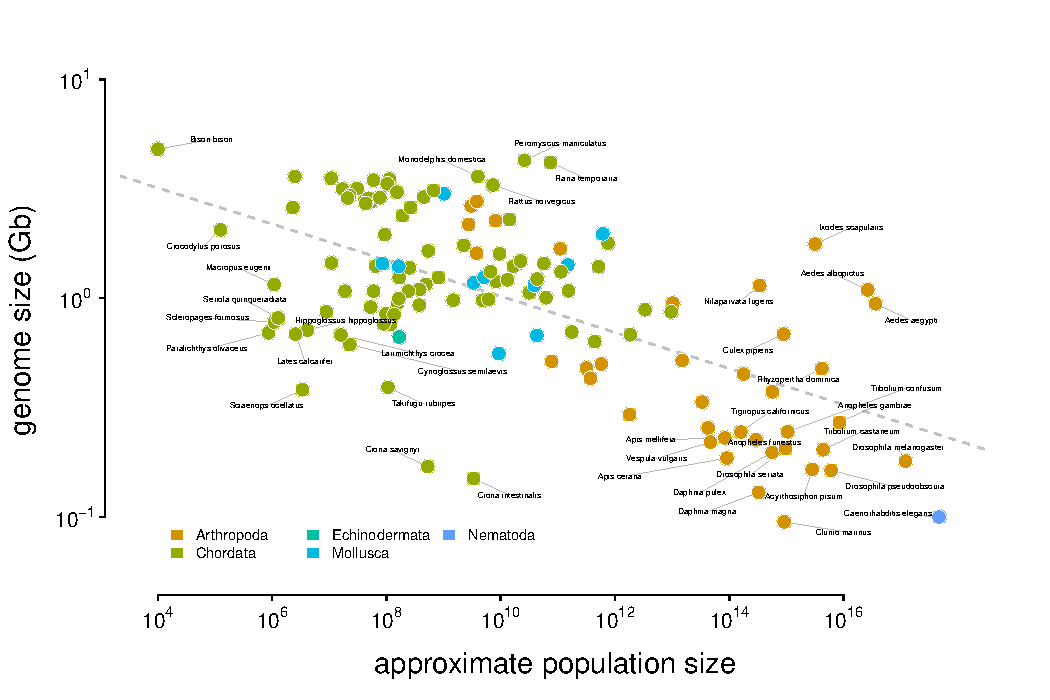
\includegraphics[width=\textwidth]{figures/genome_size_popsize.pdf}

  \caption{The relationship between genome size and approximate census
    population size. The dashed gray line indicates the OLS fit. Tiger
    salamander (\emph{Ambystoma tigrinum}) was excluded because of its
  exceptionally large genome size (~30Gbp).}

  \label{supfig:genome_size_popsize}
\end{figure}


\begin{figure}[!htb]
  \centering
  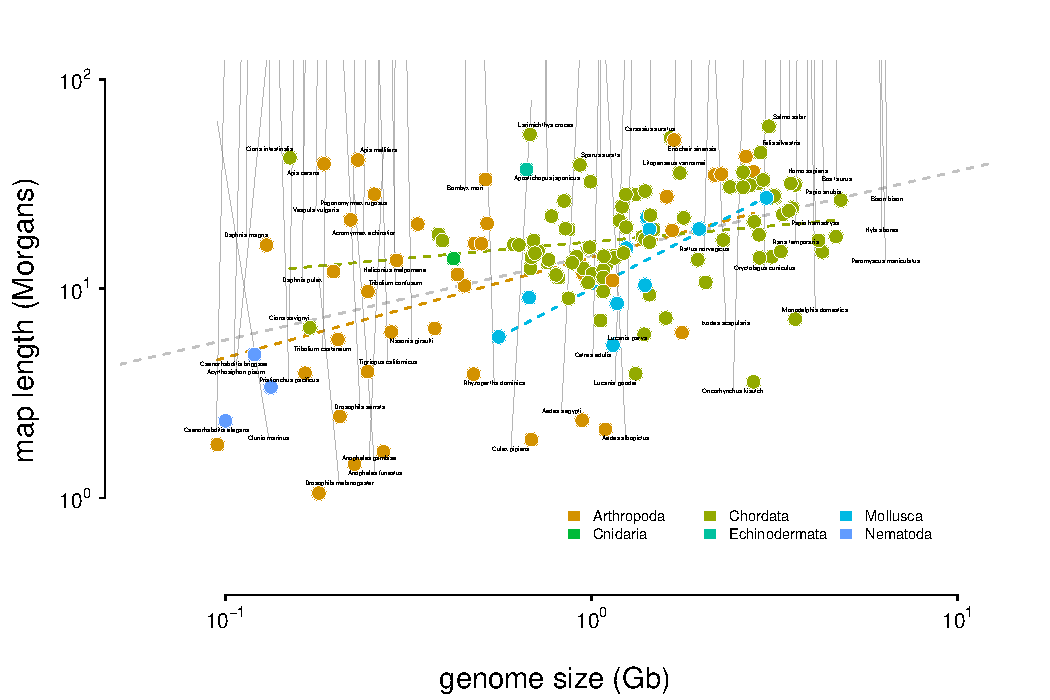
\includegraphics[width=\textwidth]{figures/genome_size_maplength.pdf}

  \caption{The relationship between genome size and recombination map length.
    The dashed gray line indicates the OLS fit for all taxa, and the dashed
    colored dashed lines indicate the linear relationship fit by phyla. Tiger
    salamander (\emph{Ambystoma tigrinum}) was excluded because of its
  exceptionally large genome size (~30Gbp).}

  \label{supfig:genome_size_maplength}
\end{figure}



\begin{figure}[!htb]
  \centering
  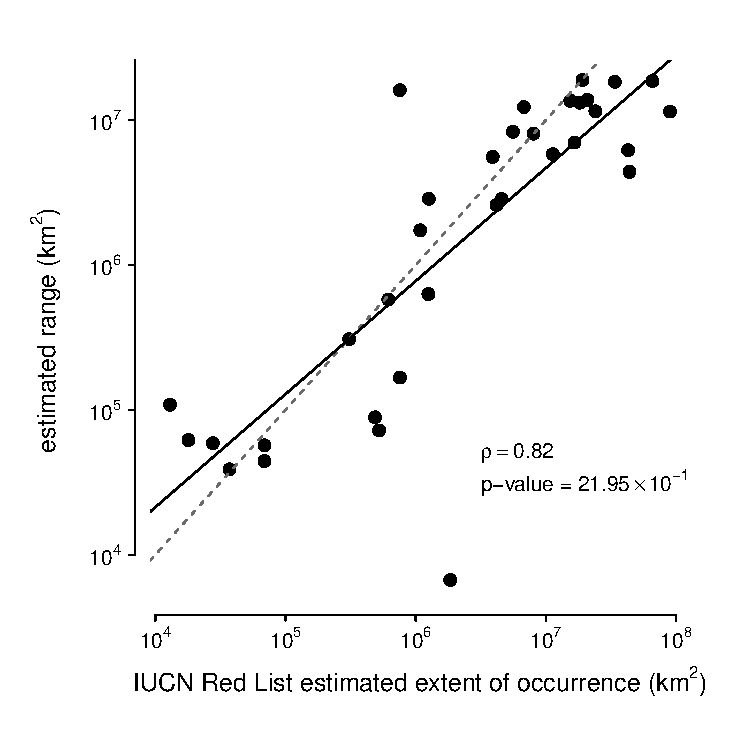
\includegraphics[]{figures/iucn_redlist_ranges.pdf}

  \caption{The correspondence between the ranges estimated with the alpha hull
    method applied to GBIF data used in this paper and IUCN Red List's Extent
    of Occurrence for the subset of species in both datasets. Note that the
    IUCN Red List contains predominantly endangered species, which leads to
    ascertainment bias; still, the high correlation between the estimated
  ranges shows the alpha hull method works well.}

  \label{suppfig:redlist-ranges}
\end{figure}

\begin{figure}[!htb]
  \centering
  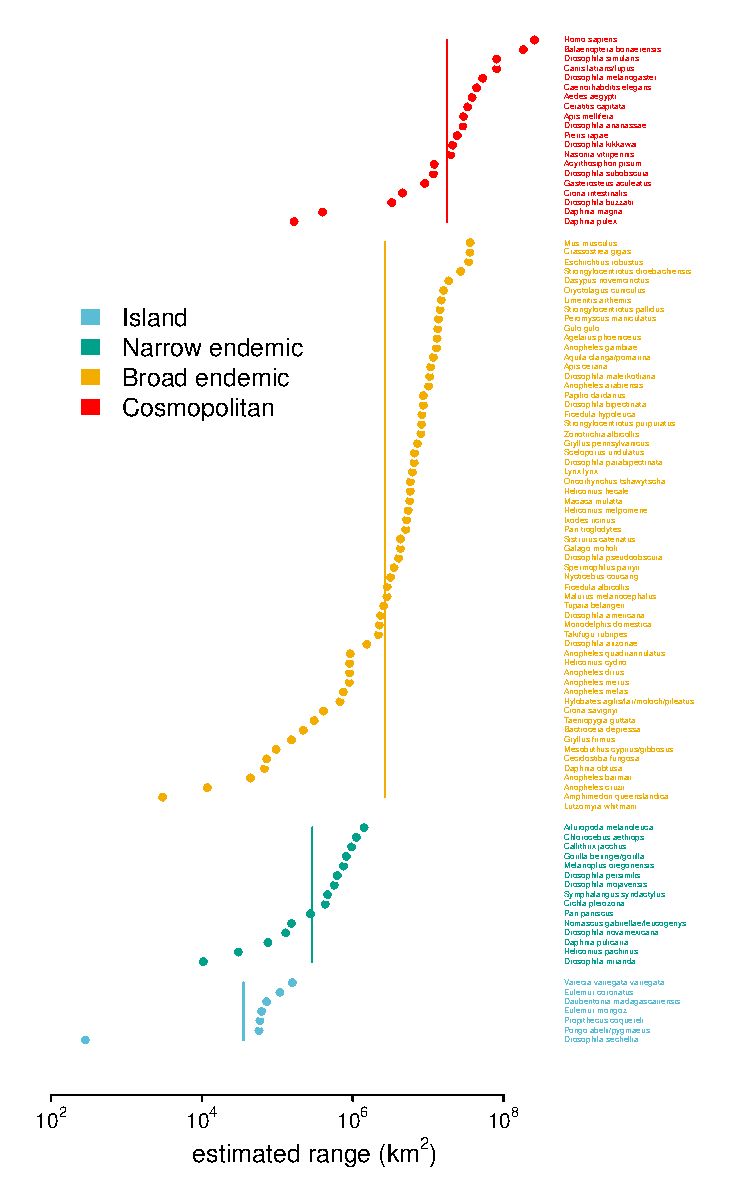
\includegraphics[]{figures/range_categories.pdf}

  \caption{The estimated ranges using GBIF occurrence data, ordered within and
    colored by the original range category labels assigned in
  \textcite{Leffler2012-zj}.}

  \label{suppfig:range-cats}
\end{figure}

\begin{figure}[!htb]
  \centering
  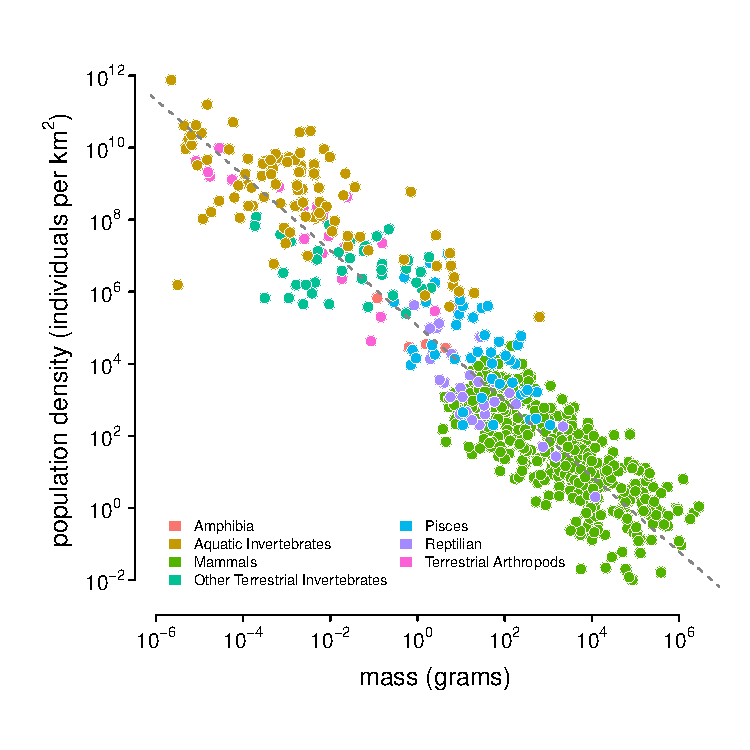
\includegraphics[]{figures/damuth.pdf}

  \caption{The appendix table of \textcite{Damuth1987-sg}; the color indicates
    Damuth's original group labels. The dashed line was estimated using a
    lognormal regression model in Stan. References to each measurement are
  available in \textcite{Damuth1987-sg}.}

  \label{suppfig:damuth}
\end{figure}

\begin{figure}[!htb]
  \centering
  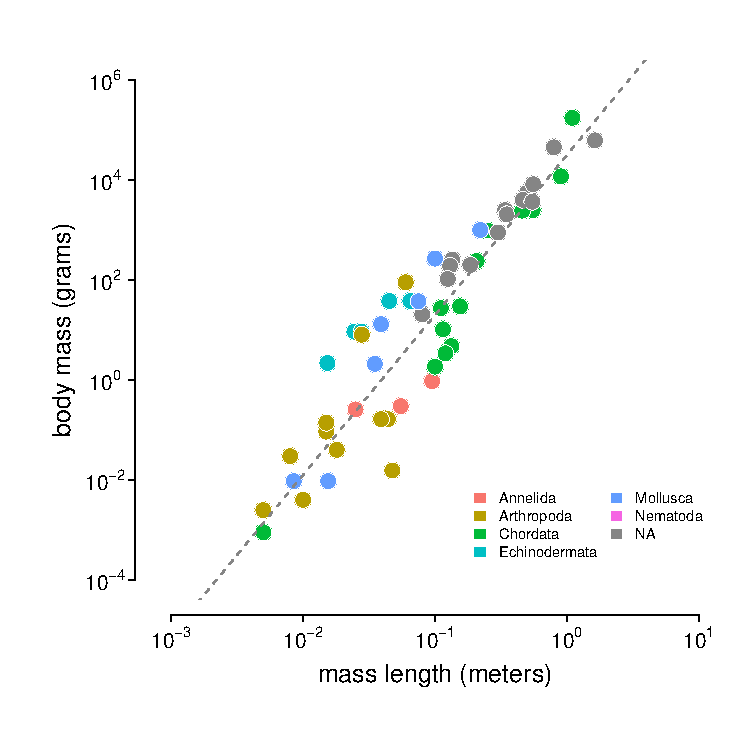
\includegraphics[]{figures/body_mass_length.pdf}

  \caption{The relationship between body length (meters) and body mass (grams)
    in the \textcite{Romiguier2014-bp} data set, used to infer body masses for
  taxa. The gray dashed line is the line of best fit inferred using Stan.}

  \label{suppfig:body-mass-length}
\end{figure}


\begin{figure}[!htb]
  \centering
  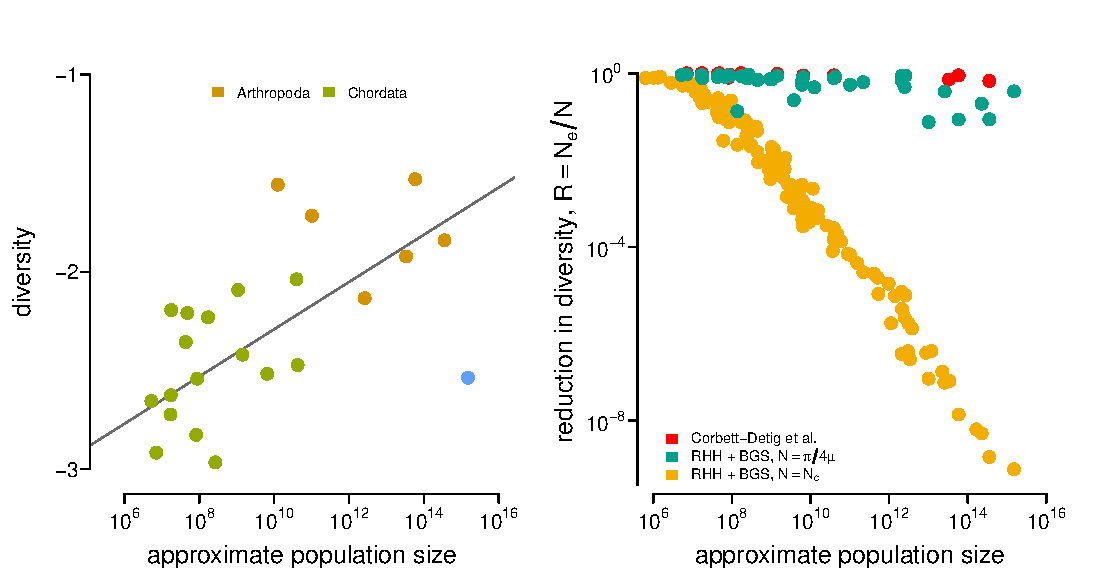
\includegraphics[width=\textwidth]{figures/corbett_detig.pdf}

  \caption{(A) The diversity data from \textcite{Corbett-Detig2015-gt} and the
    census population size estimated here for metazoan taxa. (B) The
    reductions in diversity, $R = \nicefrac{N_e}{N}$, plotted against census
    size across species. The red points are the reductions estimated by
    \textcite{Corbett-Detig2015-gt}. This confirms
    \citeauthor{Corbett-Detig2015-gt}'s (2015) finding that the impact of
    selection ($I = 1-R$) increases with census population size (though, in the
    original paper size body size and range were used as separate proxy
    variables for census population size). The green and red points are the
    predicted reduction in diversity under the recurrent hitchhiking (RHH) and
    background selection (BGS) model using the \emph{Drosophila melanogaster}
    parameters as described in the main text.  The reduction in the diversity
    due to sweeps, from Equation \eqref{eqn:div}, is determined by the term
    $2NS$.  Green points treat $N$ as the implied effective population size
    from diversity $\widetilde{N}_e = \nicefrac{\widehat{\pi}}{4\mu}$, assuming
    $\mu = 10^{-9}$. Yellow points treat $N$ as the census size, $N = N_c$.
    Overall, using the census size, e.g.  $2N_cS$, leads to reductions in
    diversity that far exceed the empirical estimates of Corbett-Detig et al.
  and reasonable model-based predictions from $\widetilde{N}_e$.}

  \label{suppfig:corbett_detig}
\end{figure}


\begin{figure}[!htb]
  \centering
  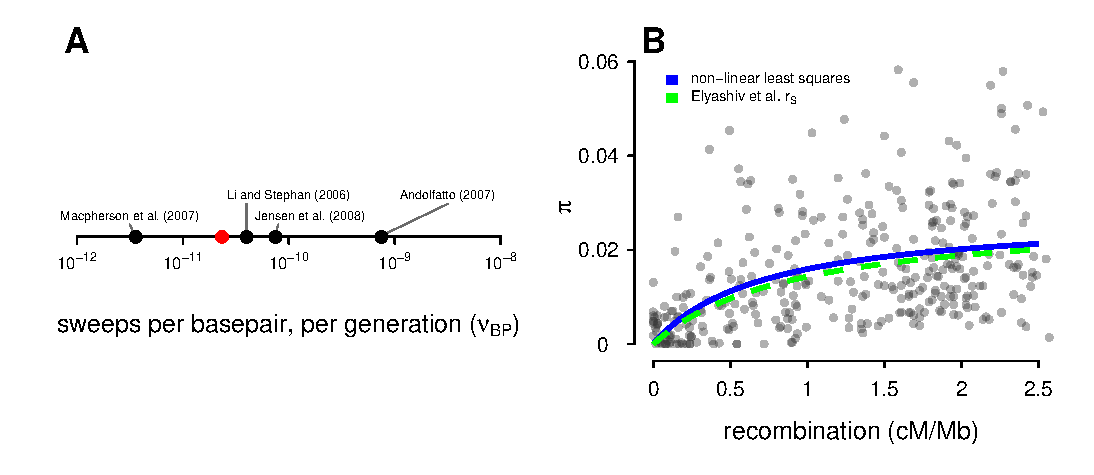
\includegraphics[width=\textwidth]{figures/linked_sel_params.pdf}

  \caption{(A) The estimate of the number of sweeps per basepair, per genome
    ($\nu_\text{BP}$) from Table 2 of \textcite{Elyashiv2016-vt} (the studies
    included are \cite{Li2006-xa,Andolfatto2007-uy,Macpherson2007-qt} and
    \cite{Jensen2008-vz}); the red point is my estimate used in
    this paper. (B) Points are the data from \textcite{Shapiro2007-gp}.  The
    blue line is the non-linear least squares fit to the data, and the green
    dashed line is the sweep model parameterized by the genome-wide average
    sweep coalescent rate $2NS \approx 0.92$ from the classic sweep and
  background selection model of \textcite{Elyashiv2016-vt} ($r_s$ in
Supplementary Table S6).}

  \label{suppfig:linked-sel-params}
\end{figure}


\begin{figure}[!htb]
  \centering
  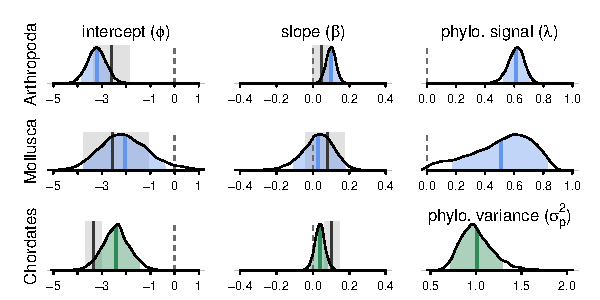
\includegraphics[width=\textwidth]{figures/div_popsize_post_phyla.pdf}

  \caption{The posterior distributions for the parameters of the phylogenetic
    mixed-effects model of diversity and population size (this is analogous to
    Figure \ref{fig:figure-2}B) fit separately on chordates ($n=68$), molluscs
    ($n=13$), and arthropods ($n=68$). The phylogenetic mixed-effects model for
    chordates indicated the best-fitting model had no residual variance
    ($\sigma_r^2 = 0$), so an alternate model without this variance component
    was used to ensure proper convergence; this model is shown in green.
    The light blue (green) shaded regions are the 90\% credible intervals, the
    blue (green) lines the posterior averages, the gray shaded regions the OLS
    bootstrap 95\% confidence intervals, and the gray lines the OLS estimate.
    Note that unlike Figure \ref{fig:figure-2}, the OLS estimate uses all taxa,
    not just those present in the phylogeny, since splitting the data by phyla
    reduces sample sizes (OLS with just the subset of taxa in the phylogeny is
    not significant for either chordates and arthropods). The vertical dashed
  gray line indicates zero.}

  \label{suppfig:div_popsize_post_phyla}
\end{figure}


\begin{figure}[!htb]
  \centering
  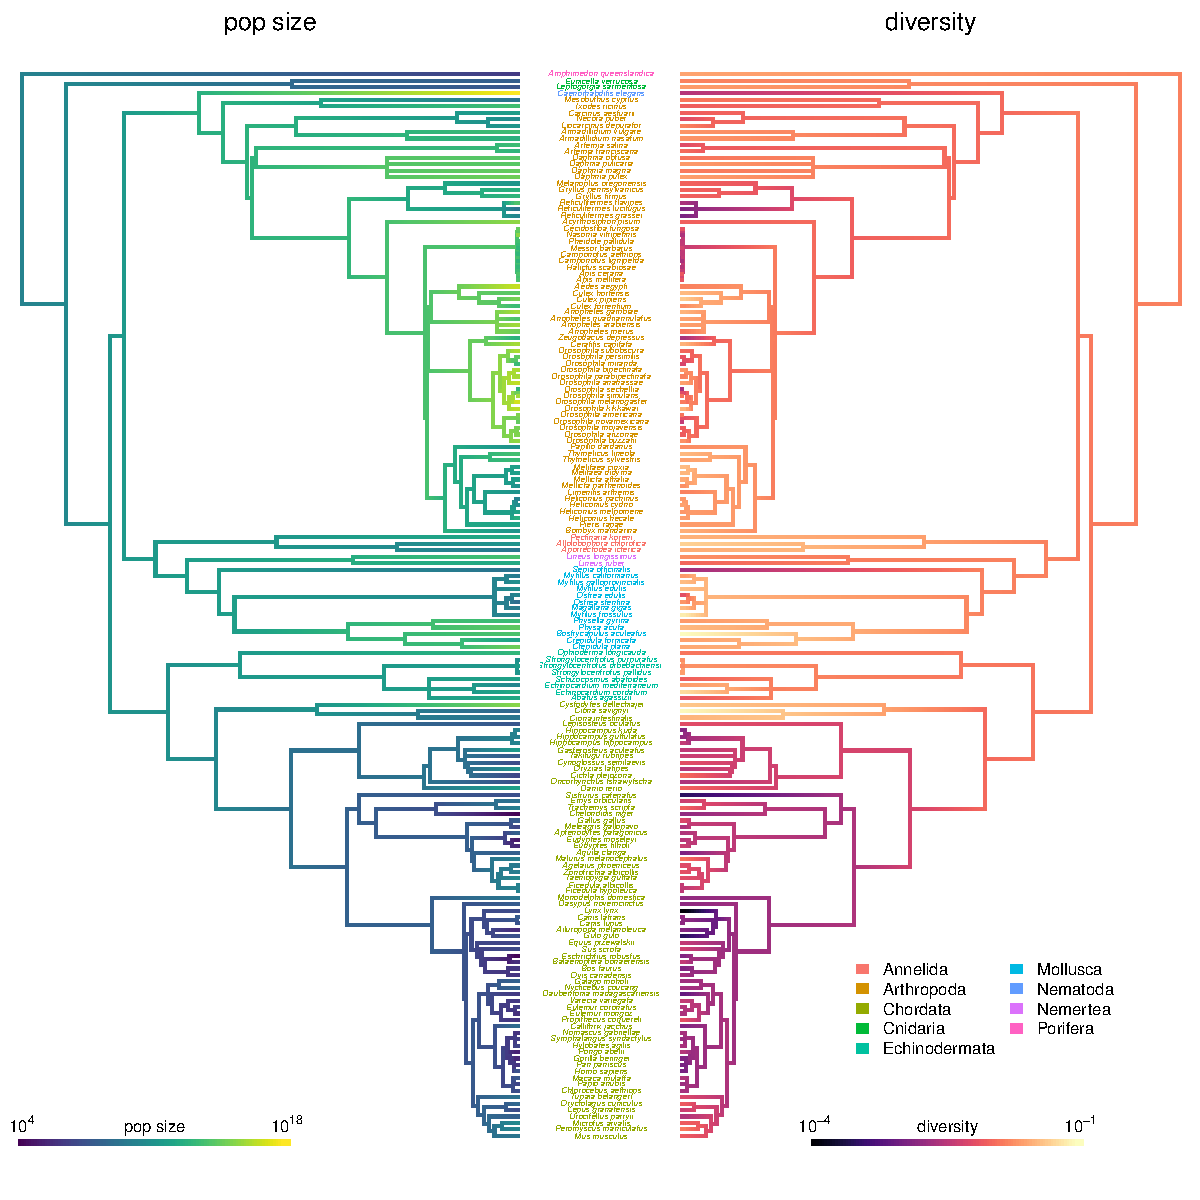
\includegraphics[width=\textwidth]{figures/biconmap_diversity.pdf}

  \caption{}

  \label{suppfig:biconmap_diversity}
\end{figure}



\begin{figure}[!htb]
  \centering
  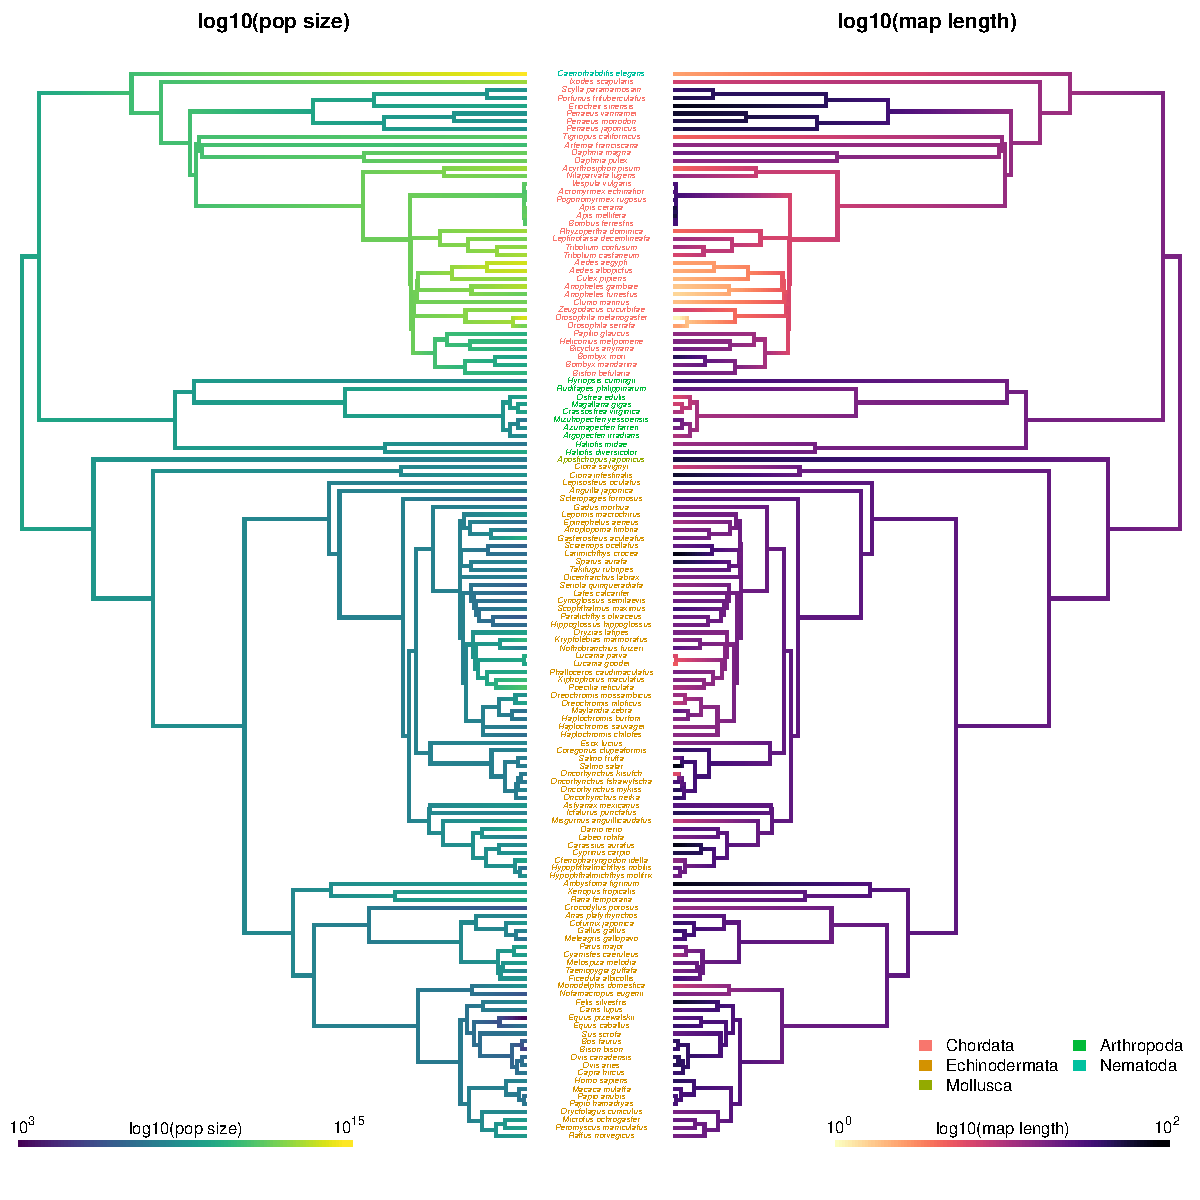
\includegraphics[width=\textwidth]{figures/biconmap.pdf}

  \caption{}

  \label{suppfig:biconmap}
\end{figure}



\end{document}

